%% abtex2-modelo-relatorio-tecnico.tex, v-1.9.6 laurocesar
%% Copyright 2012-2016 by abnTeX2 group at http://www.abntex.net.br/ 
%%
%% This work may be distributed and/or modified under the
%% conditions of the LaTeX Project Public License, either version 1.3
%% of this license or (at your option) any later version.
%% The latest version of this license is in
%%   http://www.latex-project.org/lppl.txt
%% and version 1.3 or later is part of all distributions of LaTeX
%% version 2005/12/01 or later.
%%
%% This work has the LPPL maintenance status `maintained'.
%% 
%% The Current Maintainer of this work is the abnTeX2 team, led
%% by Lauro César Araujo. Further information are available on 
%% http://www.abntex.net.br/
%%
%% This work consists of the files abntex2-modelo-relatorio-tecnico.tex,
%% abntex2-modelo-include-comandos and abntex2-modelo-references.bib
%%

% ------------------------------------------------------------------------
% ------------------------------------------------------------------------
% abnTeX2: Modelo de Relatório Técnico/Acadêmico em conformidade com 
% ABNT NBR 10719:2015 Informação e documentação - Relatório técnico e/ou
% científico - Apresentação
% ------------------------------------------------------------------------ 
% ------------------------------------------------------------------------

\documentclass[
	% -- opções da classe memoir --
	12pt,				% tamanho da fonte
	%openright,			% capítulos começam em pág ímpar (insere página vazia caso preciso)
	%twoside,           % para impressão em recto e verso. Oposto a oneside
	oneside,
	a4paper,			% tamanho do papel. 
	% -- opções da classe abntex2 --
	%chapter=TITLE,		% títulos de capítulos convertidos em letras maiúsculas
	%section=TITLE,		% títulos de seções convertidos em letras maiúsculas
	%subsection=TITLE,	% títulos de subseções convertidos em letras maiúsculas
	%subsubsection=TITLE,% títulos de subsubseções convertidos em letras maiúsculas
	% -- opções do pacote babel --
	english,			% idioma adicional para hifenização
	french,				% idioma adicional para hifenização
	spanish,			% idioma adicional para hifenização
	brazil,				% o último idioma é o principal do documento
	]{abntex2}



% PACOTES

% ---
% Pacotes fundamentais 
\usepackage{lmodern}			% Usa a fonte Latin Modern
\usepackage[T1]{fontenc}		% Selecao de codigos de fonte.
\usepackage[utf8]{inputenc}		% Codificacao do documento (conversão automática dos acentos)
\usepackage{indentfirst}		% Indenta o primeiro parágrafo de cada seção.
\usepackage{color}				% Controle das cores
\usepackage{graphicx}			% Inclusão de gráficos
\usepackage{microtype} 			% para melhorias de justificação
\usepackage{url}
% ---
\usepackage[export]{adjustbox}
% Pacotes adicionais, usados no anexo do modelo de folha de identificação
\usepackage{multicol}
\usepackage{multirow}
\usepackage{array}

\usepackage{float} % para utilizar o H de tabelas e figuras e mante-las no lugar
% ---

%----------------- PARA INSERIR ARQUIVOS DE CODIGOS -----------------%
\usepackage{xcolor}
% Definindo novas cores
\definecolor{verde}{rgb}{0,0.5,0}
% Configurando layout para mostrar codigos C++
\usepackage{listings}
\lstdefinelanguage{text}{}
\lstdefinelanguage{assembly}{}
\lstset{
  language=Verilog, %indicar a linguagem utilizada
  basicstyle=\ttfamily\tiny, 
  keywordstyle=\color{blue}, 
  stringstyle=\color{verde}, 
  commentstyle=\color{gray}, 
  extendedchars=true, 
  showspaces=false, 
  showstringspaces=false, 
  numbers=left,
  numberstyle=\tiny,
  breaklines=true, 
  backgroundcolor=\color{green!10},
  breakautoindent=true, 
  captionpos=b,
  xleftmargin=0pt,
}
% -----------------% FIM INSERIR ARQUIVOs DE CODIGO -----------------%

% Pacotes de citações
\usepackage[brazilian,hyperpageref]{backref}	 % Paginas com as citações na bibl
\usepackage[alf]{abntex2cite}	% Citações padrão ABNT
\citebrackets() %citação numérica entre colchetes
% --- 


% CONFIGURAÇÕES DE PACOTES

% Configurações do pacote backref
% Usado sem a opção hyperpageref de backref
\renewcommand{\backrefpagesname}{Citado na(s) página(s):~}
% Texto padrão antes do número das páginas
\renewcommand{\backref}{}
% Define os textos da citação
\renewcommand*{\backrefalt}[4]{
	\ifcase #1 %
		Nenhuma citação no texto.%
	\or
		Citado na página #2.%
	\else
		Citado #1 vezes nas páginas #2.%
	\fi}%
% ---

% Informações de dados para CAPA e FOLHA DE ROSTO
\titulo{Implementação de um Processador ARM-like com Integração de um Compilador C-}
\autor{Heitor Gabriel Barroso Reis}
\local{São José dos Campos - Brasil}
\data{Julho de 2025}
\instituicao{
  Docente: Prof. Dr. Luiz Eduardo Galvão Martins
  \par
  Universidade Federal de São Paulo - UNIFESP
  \par
  Instituto de Ciência e Tecnologia - Campus São José dos Campos
}
\tipotrabalho{Relatório Técnico}
\preambulo{Relatório apresentado à Universidade Federal de São Paulo como parte dos requisitos para aprovação na disciplina de Laboratório de Sistemas Computacionais: Compiladores, abordando a integração entre o processador customizado, seu conjunto de instruções e o fluxo de compilação C-.}
% ---

% Configurações de aparência do PDF final
\definecolor{blue}{RGB}{41,5,195}

\makeatletter
\hypersetup{
	pdftitle={\@title},
	pdfauthor={\@author},
	pdfsubject={\imprimirpreambulo},
	pdfcreator={LaTeX with abnTeX2},
	pdfkeywords={abnt}{latex}{abntex}{abntex2}{processador}{verilog}{fpga}{compiladores}{cminus},
	colorlinks=true,
	linkcolor=blue,
	citecolor=blue,
	filecolor=magenta,
	urlcolor=blue,
	bookmarksdepth=4,
	hypertexnames=false
}
\makeatother
% ---

% Espaçamentos entre linhas e parágrafos
\setlength{\parindent}{1.3cm}
\setlength{\parskip}{0.2cm}

\makeindex
% ---

% ------------------------------------------------
% Início do documento
\begin{document}

\selectlanguage{brazil}
\frenchspacing

% ----------------------------------------------------------
% ELEMENTOS PRÉ-TEXTUAIS
% ----------------------------------------------------------
\imprimircapa
\imprimirfolhaderosto*

% ---
% RESUMO
\setlength{\absparsep}{18pt}
\begin{resumo}
    Este relatório apresenta o projeto integrado de um sistema computacional didático, composto por um processador customizado de 32 bits e por um compilador C- acrescentado ao fluxo de desenvolvimento para gerar programas executáveis para essa arquitetura. O processador, descrito em Verilog na versão \texttt{Processor(v2026-1)}, adota uma organização RISC ARM-like, arquitetura Harvard, instruções de 32 bits, execução condicional por flags, banco de registradores, ROM de instruções, RAM de dados e interfaces de entrada e saída para testes em FPGA e simulação. Sobre essa base, o compilador foi integrado como ferramenta de apoio ao processador: ele analisa programas C- com um front-end em C usando Flex e Bison, constrói AST e tabela de símbolos, executa análise semântica, gera IR, traduz o programa por um back-end em Python para assembly da arquitetura e monta o código binário de 32 bits carregável na ROM. O documento descreve tanto a organização do hardware quanto o pipeline de compilação, destacando o contrato entre formato de instruções, memória, chamadas de função, simulador, arquivos gerados pelo compilador e exemplos de execução. Dessa forma, o compilador não é tratado como um artefato isolado, mas como uma extensão do projeto do processador, responsável por tornar a programação e a validação do sistema mais sistemáticas.

    \noindent
    \textbf{Palavras-chaves}: Processador. Verilog. FPGA. Compiladores. C-. Arquitetura ARM-like. RISC. Geração de Código.
\end{resumo}

% ---
% LISTAS
\pdfbookmark[0]{\listfigurename}{lof}
\listoffigures*
\clearpage

\pdfbookmark[0]{\listtablename}{lot}
\listoftables*
\clearpage
% ---

% ---
% SUMÁRIO
\pdfbookmark[0]{\contentsname}{toc}
\tableofcontents*
% ---

% ----------------------------------------------------------
% ELEMENTOS TEXTUAIS
% ----------------------------------------------------------
\textual

% ----------------- Introdução -------------------------------
\chapter{Introdução}

Um processador didático só se torna plenamente verificável quando existe um caminho claro entre o algoritmo escrito pelo programador, as instruções aceitas pela arquitetura e a execução observada no hardware \cite{patterson2017,compOrgDes}. Este relatório apresenta esse caminho para um processador customizado de 32 bits, baseado em princípios RISC e inspirado na arquitetura ARM (\emph{Advanced RISC Machine}), ao qual foi integrado um compilador para a linguagem C-, um subconjunto da linguagem C.

O trabalho parte do processador desenvolvido na disciplina de Arquitetura e Organização de Computadores e o atualiza como uma plataforma completa de execução. Nessa plataforma, o compilador não substitui a descrição do hardware: ele é adicionado ao projeto para automatizar a geração de programas compatíveis com o conjunto de instruções, com a organização de memória e com os sinais efetivamente implementados no \texttt{Processor(v2026-1)}.

O fluxo integrado segue a cadeia código-fonte C-, análise léxica, análise sintática, AST, tabela de símbolos, análise semântica, IR, assembly e código binário.

O Capítulo \ref{cap:processador} descreve a arquitetura do processador, seu formato de instruções e os pontos atualizados da versão \texttt{Processor(v2026-1)}. O Capítulo \ref{cap:analise} aborda a fase de análise do compilador adicionado ao sistema. O Capítulo \ref{cap:sintese} detalha a fase de síntese, incluindo a geração de código intermediário, assembly e código de máquina compatível com o processador. O Capítulo \ref{cap:exemplos} apresenta exemplos práticos de execução do fluxo completo, e o Capítulo \ref{cap:conclusao} conclui o relatório com as dificuldades encontradas e os principais destaques do projeto integrado.

%---------------- O Processador -------------------------------------
\chapter{O Processador}
\label{cap:processador}
O processador é a base do sistema descrito neste relatório. Trata-se de uma arquitetura customizada de 32 bits, fortemente inspirada no conjunto de instruções e na filosofia de design da ARM (\emph{Advanced RISC Machine}), adaptada a uma finalidade didática e à implementação em FPGA. Este processador foi inicialmente modelado a partir de referências da arquitetura ARM presentes no \emph{DataSheet} oficial \cite{ARM_Datasheet,ARMtechnical}. Na versão atual do projeto, a referência prática é o \texttt{Processor(v2026-1)}, descrito em Verilog e organizado como um projeto Quartus para o dispositivo Cyclone IV E \texttt{EP4CE115F29C7}. O compilador C- foi adicionado a essa base para gerar programas para o processador; por isso, ele não emite código ARM comercial, mas uma codificação ARM-like simplificada, ajustada aos campos, memórias e sinais realmente implementados no hardware do projeto.

\section{Arquitetura e Organização}

O processador segue a filosofia \textbf{RISC (\emph{Reduced Instruction Set Computer})}, caracterizada por um conjunto de instruções simples, de largura fixa, com campos regulares para registradores, imediato e função \cite{patterson2017,stallings2017}. Adota-se a \textbf{arquitetura Harvard}, que utiliza memórias separadas para instruções (ROM) e dados (RAM) \cite{compOrgDes,compArchi}. No \texttt{Processor(v2026-1)}, a memória de instruções possui 1024 palavras de 32 bits e é inicializada pelo arquivo de inicialização da ROM; a memória de dados possui 64 palavras de 32 bits.

Uma característica notável herdada da ARM é a \textbf{execução condicional}. Todas as instruções possuem um campo de 4 bits (\texttt{Cond}) que permite que sua execução seja dependente do estado de flags armazenadas no registrador de status \textbf{CPSR (\emph{Current Program Status Register})}. Na implementação atual, as flags efetivamente usadas pelo verificador de condição são Z (Zero) e N (Negative); os campos C e V permanecem como parte conceitual do modelo ARM, mas não são a base das decisões do compilador.

\begin{table}[H]
    \centering
    \ABNTEXfontereduzida
    \caption{Campos da instrução de 32 bits usada pelo \texttt{Processor(v2026-1)}}
    \label{tab:campos_instrucao_processor}
    \begin{tabular}{|p{0.18\textwidth}|p{0.18\textwidth}|p{0.52\textwidth}|}
        \hline
        \textbf{Campo} & \textbf{Bits} & \textbf{Função no processador} \\
        \hline
        \texttt{Cond} & \texttt{[31:28]} & Seleciona a condição de execução verificada contra as flags Z/N. \\
        \hline
        \texttt{Type} & \texttt{[27:26]} & Define a classe: processamento de dados, load/store ou branch. \\
        \hline
        \texttt{Supp} & \texttt{[25:24]} & Indica uso de imediato e/ou atualização de flags. \\
        \hline
        \texttt{Funct} & \texttt{[23:20]} & Seleciona a operação dentro da classe e, em branches, ativa link ou retorno por link. \\
        \hline
        \texttt{Rd} & \texttt{[19:15]} & Registrador destino. \\
        \hline
        \texttt{Rh} & \texttt{[14:10]} & Registrador fonte/base. \\
        \hline
        \texttt{Operand2} & \texttt{[9:0]} & Imediato assinado de 10 bits ou registrador \texttt{Ro} em \texttt{[9:5]}. \\
        \hline
    \end{tabular}
    \legend{Fonte: O autor, com base no RTL do \texttt{Processor(v2026-1)}.}
\end{table}

\subsection{CPSR e Sufixos de Instruções}
Na arquitetura ARM, o CPSR é um registrador dedicado a salvar um conjunto de estados de um resultado de instrução. As \emph{flags} são características de estado do resultado e são expressas pelos \emph{bits} N (Negative), Z (Zero), C (Carry) e V (Overflow). Para o programador, as condições de execução são definidas por meio de um sufixo específico para cada condição, que é traduzido pelo montador para o campo \texttt{Cond} da instrução \cite{ARMtechnical,siteCPSR}. Este processador implementou um CPSR de 4 bits, com as flags Z (Zero) e N (Negative) sendo utilizadas.

\begin{figure}[H]
    \centering
    \caption{Formato de \emph{Condition Field} e sua condição correspondente}
    \label{fig:cond_field_codes}
    \graphicspath{ {./Imagens/} }
    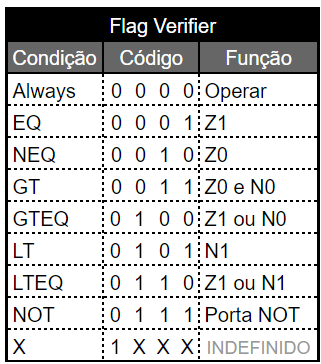
\includegraphics[scale=0.5]{cond_field_codes.png}
    \legend{Na imagem, a coluna "Função" mostra quais \emph{flags} são verificadas. Por exemplo, "Z1" representa \emph{flag} Z em nível alto. Fonte: O autor.}
\end{figure}

Além dos sufixos de condição, existem os \textbf{Sufixos de Suporte} que alteram o funcionamento da instrução:
\begin{itemize}
    \item \textbf{\texttt{i} (Imediato):} Indica que o segundo operando é um valor numérico imediato (de até 10 bits), em vez de um valor contido em um registrador.
    \item \textbf{\texttt{s} (Set CPSR):} Indica que a instrução deve atualizar as flags do CPSR com base no seu resultado.
\end{itemize}

\section{Componentes Principais e Caminho de Dados}

O caminho de dados (\emph{datapath}) foi adaptado do modelo MIPS clássico para incorporar os elementos exclusivos da arquitetura ARM, como o CPSR e a lógica de execução condicional \cite{patterson2017,compOrgDes}.

\begin{figure}[H]
    \centering
    \caption{Caminho de dados projetado}
    \label{fig:DataPathSingleCycle}
    \graphicspath{ {./Imagens/} }
    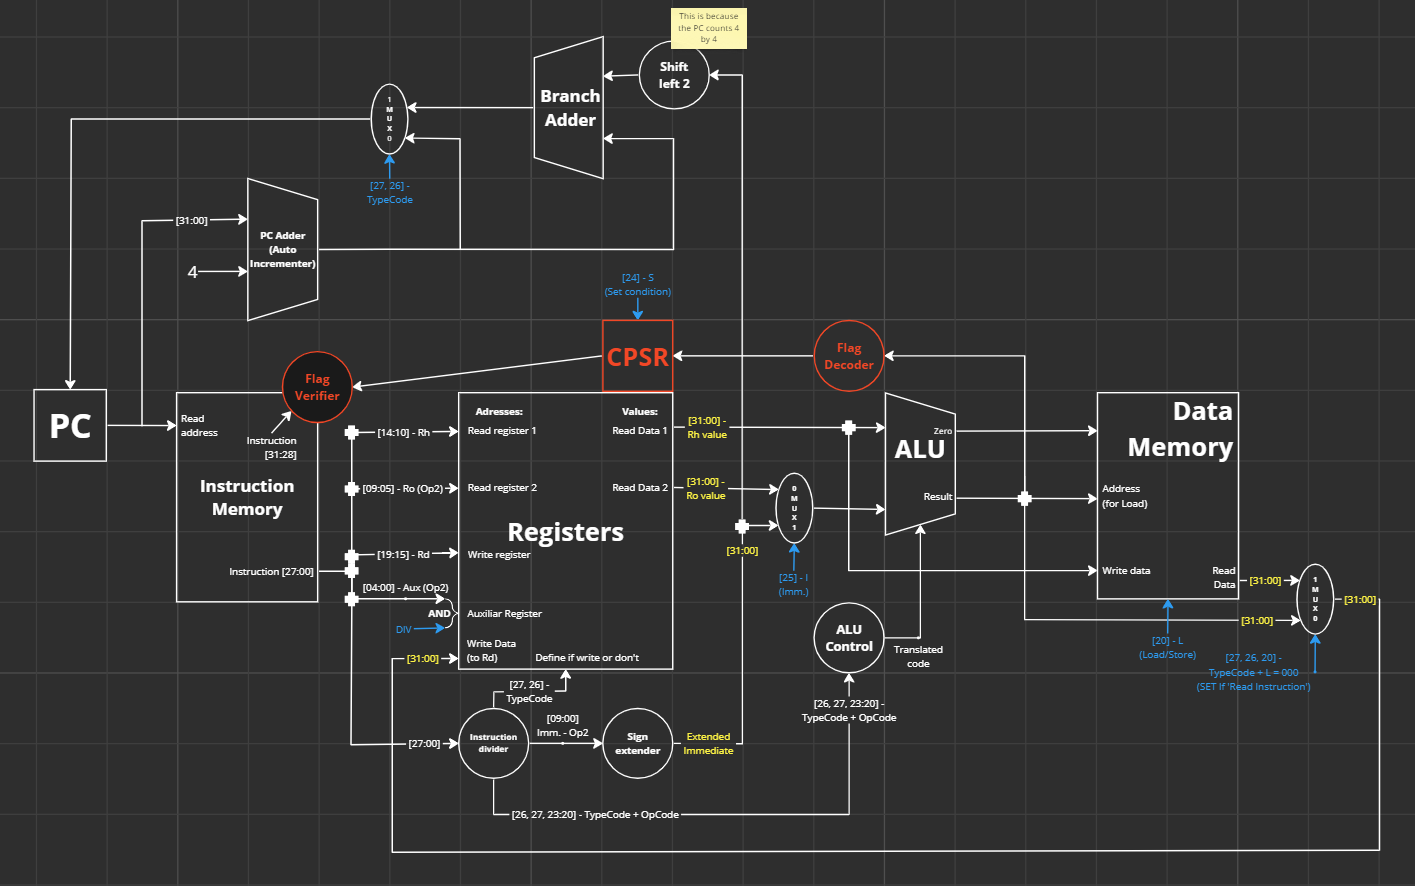
\includegraphics[scale=0.5]{DataPathSingleCycle.png}
    \legend{Caminho de dados adaptado do modelo MIPS para conter os elementos da arquitetura ARM. Fonte: O autor.}
\end{figure}

Os principais componentes são:
\begin{itemize}
    \item \textbf{Unidade de Controle (UC):} Adicionada para servir como um centro de distribuição de códigos de instruções e endereços de registradores, funcionando como um gestor de tarefas.
    \item \textbf{Banco de Registradores:} Apresenta 32 registradores de 32 bits de uso geral e um registrador de link dedicado. No RTL atual, escritas em registradores gerais e no link ocorrem na subida do \emph{clock}, enquanto as saídas de leitura são atualizadas no \texttt{fast\_clock}.
    \item \textbf{Unidade Lógica e Aritmética (ULA):} Realiza operações de Processamento de Dados como adição, subtração, multiplicação, divisão e operações lógicas (AND, OR, XOR, NOT). Também é utilizada como intermédio em operações de Transferência de Dados e Ramo.
    \item \textbf{Memória de Instruções (ROM):} Armazena o programa a ser executado, sendo acessada utilizando o PC como índice. A ROM possui 1024 palavras de 32 bits e carrega seu conteúdo por \texttt{\$readmemb} a partir de \texttt{single\_port\_rom\_init.txt}.
    \item \textbf{Memória de Dados (RAM):} Armazenamento utilizado por operações de transferência de dados. Possui 64 palavras de 32 bits, escreve na subida do \emph{clock} e atualiza a saída de leitura no \texttt{fast\_clock}.
    \item \textbf{Contador de Programa (PC):} Indica à memória de instrução qual instrução está sendo executada no momento. É atualizado a cada descida de \emph{clock}.
    \item \textbf{Módulos de Flags (CPSR, Flag Verifier, Flag Decoder):} Gerenciam a lógica de execução condicional. O \emph{Flag Verifier} compara a condição da instrução com o estado do CPSR, enquanto o \emph{Flag Decoder} interpreta o resultado das operações para salvar no CPSR.
\end{itemize}

\begin{table}[H]
    \centering
    \ABNTEXfontereduzida
    \caption{Interface externa relevante para testes do \texttt{Processor(v2026-1)}}
    \label{tab:interface_processor}
    \begin{tabular}{|p{0.24\textwidth}|p{0.62\textwidth}|}
        \hline
        \textbf{Sinal} & \textbf{Uso no projeto} \\
        \hline
        \texttt{SW[16]} & Reset do processador e do detector de entrada. \\
        \hline
        \texttt{SW[15]} & Sinal periférico usado por \texttt{in}; quando a execução está temporariamente parada, a liberação ocorre na transição de descida \texttt{1 -> 0}. \\
        \hline
        \texttt{SW[17]} & Pausa o \emph{clock} efetivo quando está em nível alto. \\
        \hline
        \texttt{SW[7:0]} & Valor de entrada fornecido à instrução \texttt{in}. \\
        \hline
        \texttt{LEDR[0]} & Expõe \texttt{write\_condition}, isto é, o resultado da verificação de condição pelo CPSR. \\
        \hline
        \texttt{output\_value} & Último valor emitido por \texttt{out}. \\
        \hline
        \texttt{pc} & Endereço da instrução corrente. \\
        \hline
    \end{tabular}
    \legend{Fonte: O autor, com base em \texttt{Processor.v} e \texttt{integrated.v}.}
\end{table}

\section{Conjunto de Instruções}

As instruções de 32 bits são divididas em três tipos principais, definidos por um campo \texttt{TypeCode} de 2 bits. O formato foi refinado durante o projeto para reduzir ambiguidades e aumentar o número de funcionalidades \cite{ARM_Datasheet,ARMtechnical}.

\begin{figure}[H]
    \centering
    \caption{Formato de Instruções ARM implementado}
    \label{fig:instSetVersion2}
    \graphicspath{ {./Imagens/} }
    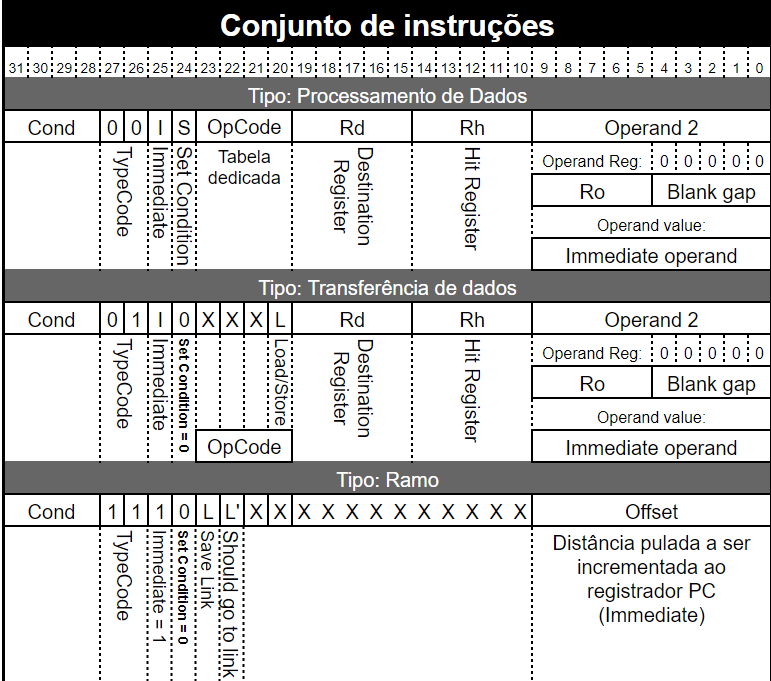
\includegraphics[scale=0.5]{instSetVersion2.png}
    \legend{Versão final implementada do formato de instruções. Fonte: O autor.}
\end{figure}

\begin{enumerate}
    \item \textbf{Processamento de Dados (Type 00):} Realiza operações aritméticas e lógicas. Inclui instruções como \texttt{ADD}, \texttt{SUB}, \texttt{MUL}, \texttt{DIV}, \texttt{AND}, \texttt{OR}, \texttt{MOV} e \texttt{IN} (entrada periférica).
    \item \textbf{Transferência de Dados (Type 01):} Move dados entre o banco de registradores e a memória. As instruções são \texttt{Load} (carregar da memória) e \texttt{Store} (armazenar na memória), diferenciadas pelo bit L do OpCode. No RTL atual e no código gerado pelo compilador, o endereço efetivo é fornecido por registrador.
    \item \textbf{Ramo (Branch) (Type 11):} Altera o fluxo de controle do programa. A instrução \texttt{B} realiza um desvio, enquanto \texttt{BL} (Branch with Link) salva o endereço de retorno, sendo essencial para chamadas de função.
\end{enumerate}

Na versão \texttt{Processor(v2026-1)}, a lógica de desvio foi refinada para separar claramente três formas de destino: deslocamento imediato relativo ao PC, destino absoluto em registrador geral e retorno pelo registrador de link dedicado. Essa distinção é importante para o compilador, pois o montador pode expandir desvios longos carregando o endereço absoluto em um registrador e emitindo um branch por registrador.

\begin{table}[H]
    \centering
    \ABNTEXfontereduzida
    \caption{Semântica atual das instruções de branch no \texttt{Processor(v2026-1)}}
    \label{tab:branch_processor}
    \begin{tabular}{|p{0.21\textwidth}|p{0.23\textwidth}|p{0.38\textwidth}|}
        \hline
        \textbf{Classe} & \textbf{Bits relevantes} & \textbf{Comportamento quando a condição passa} \\
        \hline
        Branch imediato & \texttt{Type=11}, \texttt{i=1}, \texttt{Funct[22]=0} & \texttt{PC := PC + immediate}. \\
        \hline
        Branch por registrador & \texttt{Type=11}, \texttt{i=0}, \texttt{Funct[22]=0} & \texttt{PC := RoValue}. Não é mais \texttt{PC + registrador}. \\
        \hline
        Branch-and-link imediato & \texttt{Funct[23]=1}, \texttt{i=1}, \texttt{Funct[22]=0} & \texttt{Link := PC+1}; depois \texttt{PC := PC + immediate}. \\
        \hline
        Branch-and-link por registrador & \texttt{Funct[23]=1}, \texttt{i=0}, \texttt{Funct[22]=0} & \texttt{Link := PC+1}; depois \texttt{PC := RoValue}. \\
        \hline
        Retorno por link dedicado & \texttt{Type=11}, \texttt{Funct[22]=1} & \texttt{PC := LinkValue}. \\
        \hline
    \end{tabular}
    \legend{Fonte: O autor, com base em \texttt{ControlUnit.v}, \texttt{registerBank.v} e \texttt{PC\_main.v}.}
\end{table}

\section{Organização da Memória}

O processador possui um espaço de endereçamento de 32 bits e adota a arquitetura Harvard, com memórias distintas:
\begin{itemize}
    \item \textbf{Memória de Instruções (ROM):} Guarda as palavras de instrução do programa em ordem. O montador do compilador gera o código de máquina final; para execução no projeto Quartus, esse conteúdo deve alimentar o arquivo de inicialização da ROM.
    \item \textbf{Memória de Dados (RAM):} Possui 64 palavras de 32 bits. Para o compilador, esta memória é usada por uma pilha lógica de 64 palavras, inicializada com \texttt{sp = 63}, e por regiões de dados acessadas por endereço. Variáveis locais, parâmetros e temporários derramados são endereçados em relação a \texttt{fp} (\emph{Frame Pointer}); valores globais são materializados por diretivas na seção \texttt{.data}.
\end{itemize}

Essa organização exige que o compilador seja conservador no uso de memória: chamadas recursivas, vetores e muitos temporários competem por uma RAM pequena. Por isso, a validação pelo simulador de código de máquina é útil antes de carregar o programa no processador, pois permite observar PC, registradores, flags, link e memória final em um relatório textual.

%------------------- Fase de Análise -------------------
\chapter{Compilador: Fase de Análise}
\label{cap:analise}

Depois de definida a arquitetura alvo, o projeto passou a contar com um compilador C- para facilitar a criação de programas executáveis no processador. Este capítulo detalha a fase de análise desse compilador, responsável por validar a estrutura e o significado do código-fonte antes que qualquer instrução seja gerada para o hardware. Esta fase é dividida nas etapas de análise léxica, sintática e semântica, que trabalham em conjunto para transformar o código em uma representação estruturada, como a Árvore Sintática Abstrata (AST), e validar sua correção, seguindo o modelo clássico de organização de compiladores \cite{compiladoresLouden}. O front-end do compilador, responsável por esta fase, foi desenvolvido em C utilizando as ferramentas Flex e Bison.

Do ponto de vista de implementação, a fase de análise não é um bloco único. Ela é formada por módulos pequenos, cada um com uma responsabilidade bem definida. A documentação interna dos módulos do compilador detalha essas funções; a \autoref{tab:modulos_frontend} resume os grupos que mais influenciam o comportamento do compilador.

\begin{table}[H]
    \centering
    \ABNTEXfontereduzida
    \caption{Agrupamento dos módulos da fase de análise}
    \label{tab:modulos_frontend}
    \begin{tabular}{|p{0.23\textwidth}|p{0.25\textwidth}|p{0.36\textwidth}|}
        \hline
        \textbf{Grupo} & \textbf{Arquivos} & \textbf{Função principal} \\
        \hline
        Orquestração & \texttt{main.c} & Abre o arquivo, inicializa escopos e símbolos nativos, chama parser, semântica e escrita dos artefatos. \\
        \hline
        Estado de análise & \texttt{analysis\_state.c/h} & Separa erros léxicos e sintáticos, evitando mensagens em cascata. \\
        \hline
        Léxico e parser & \texttt{lexer.l}, \texttt{parser.y} & Reconhece tokens com Flex, aplica a gramática C- com Bison, registra declarações iniciais e constrói a AST. \\
        \hline
        AST & \texttt{syntax\_tree.c/h} & Cria, encadeia, imprime e libera nós sintáticos usados pela semântica e pelo gerador de IR. \\
        \hline
        Escopos e símbolos & \texttt{utils.c/h}, \texttt{symbol\_table.c/h} & Controla escopo global, funções, blocos aninhados, declarações, usos e assinaturas. \\
        \hline
        Semântica & \texttt{semantic.c/h} & Valida tipos, redeclarações, vetores, chamadas, retorno e presença de \texttt{main}. \\
        \hline
    \end{tabular}
    \legend{Fonte: O autor.}
\end{table}

\section{Modelagem}

A modelagem da fase de análise foi realizada utilizando diagramas de blocos e de atividades SysML para visualizar a estrutura e o fluxo de cada etapa.

\begin{figure}[H]
    \centering
    \caption{Diagrama de Blocos da Análise Léxica}
    \graphicspath{ {./Imagens/} }
    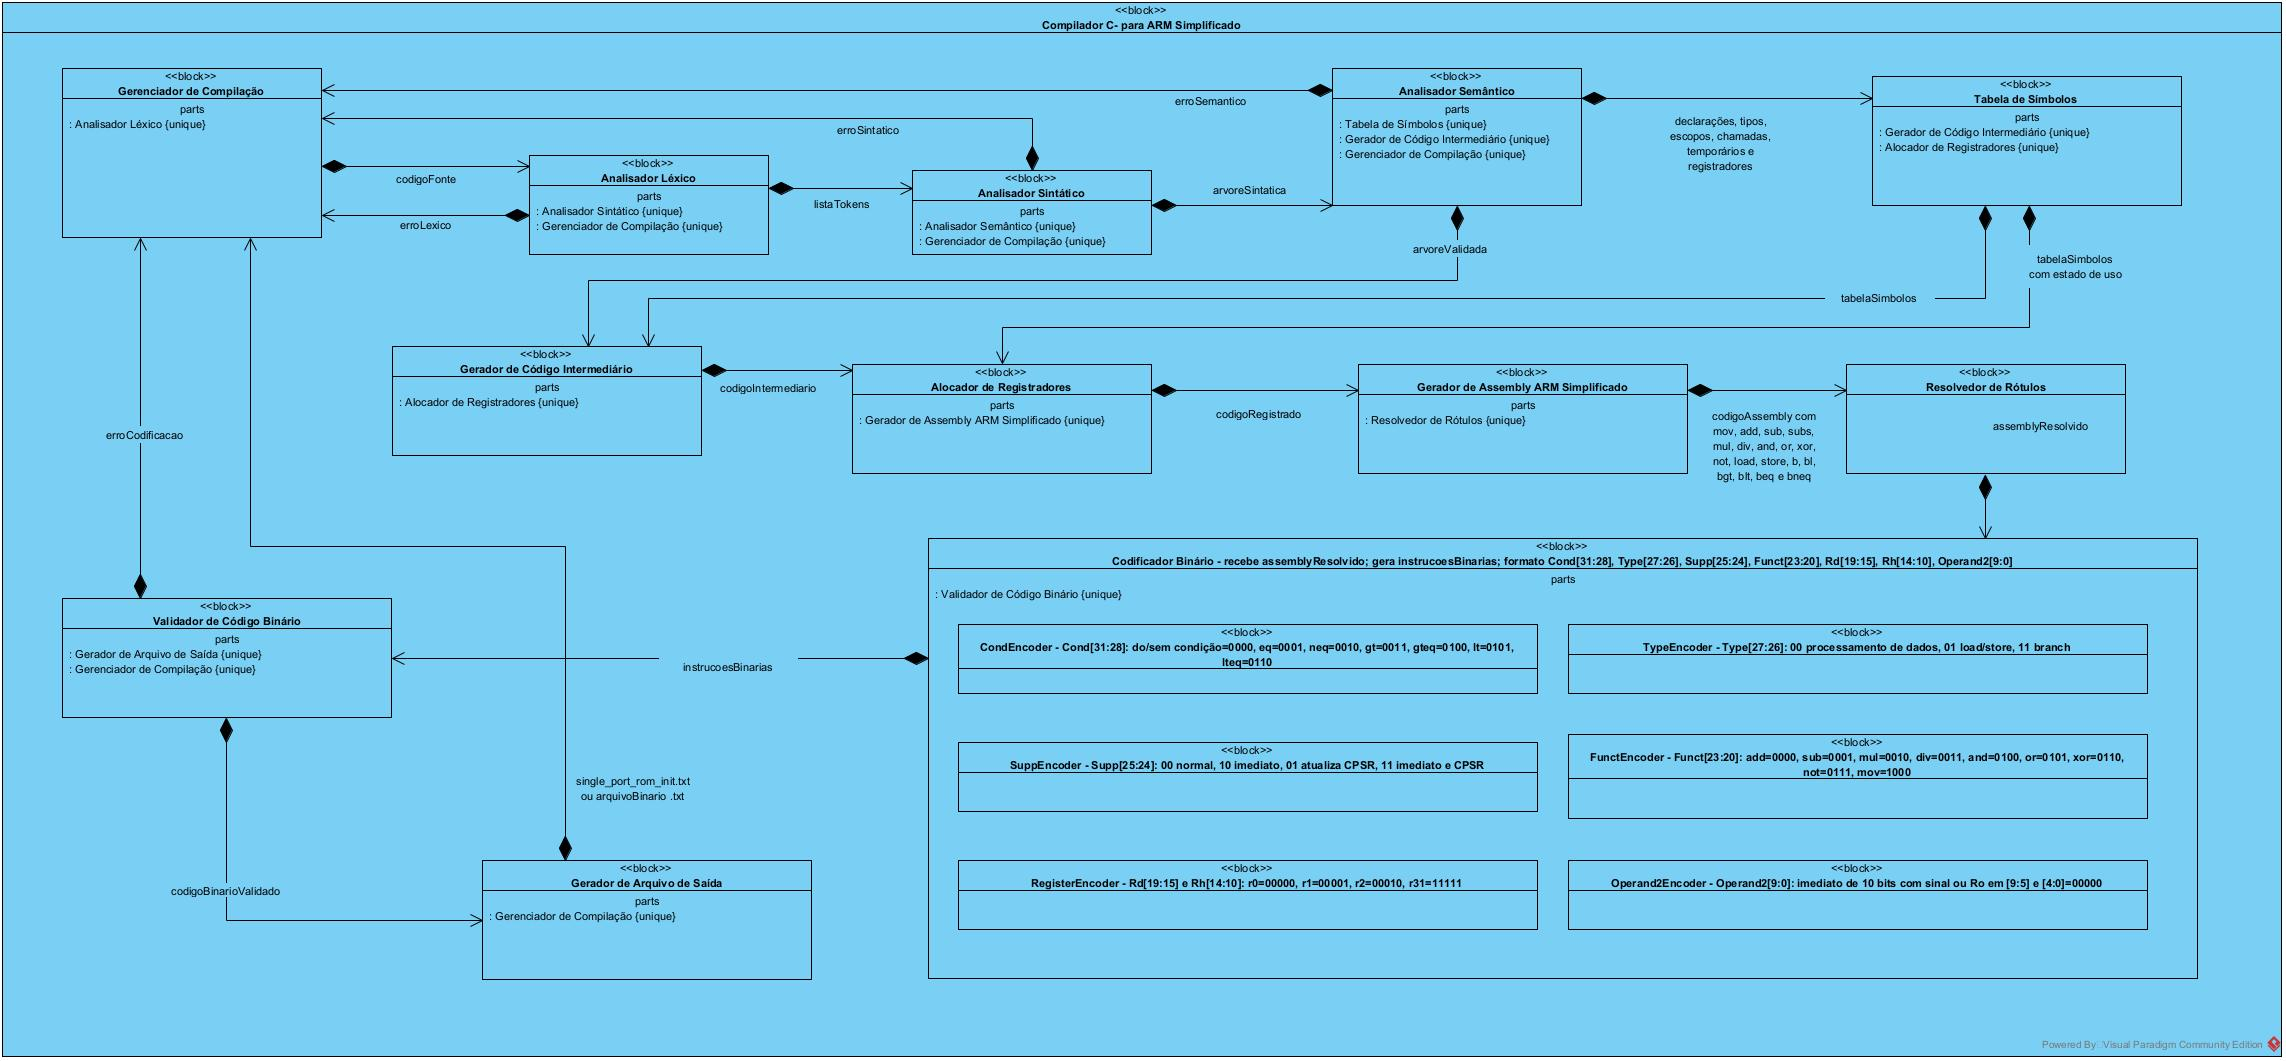
\includegraphics[width=0.8\textwidth]{Diagrama de Blocos - Arquitetura Interna do Compilador.jpg}
    \legend{Fonte: O autor.}
\end{figure}

\begin{figure}[H]
    \centering
    \caption{Diagrama de Atividades da Análise Léxica}
    \graphicspath{ {./Imagens/} }
    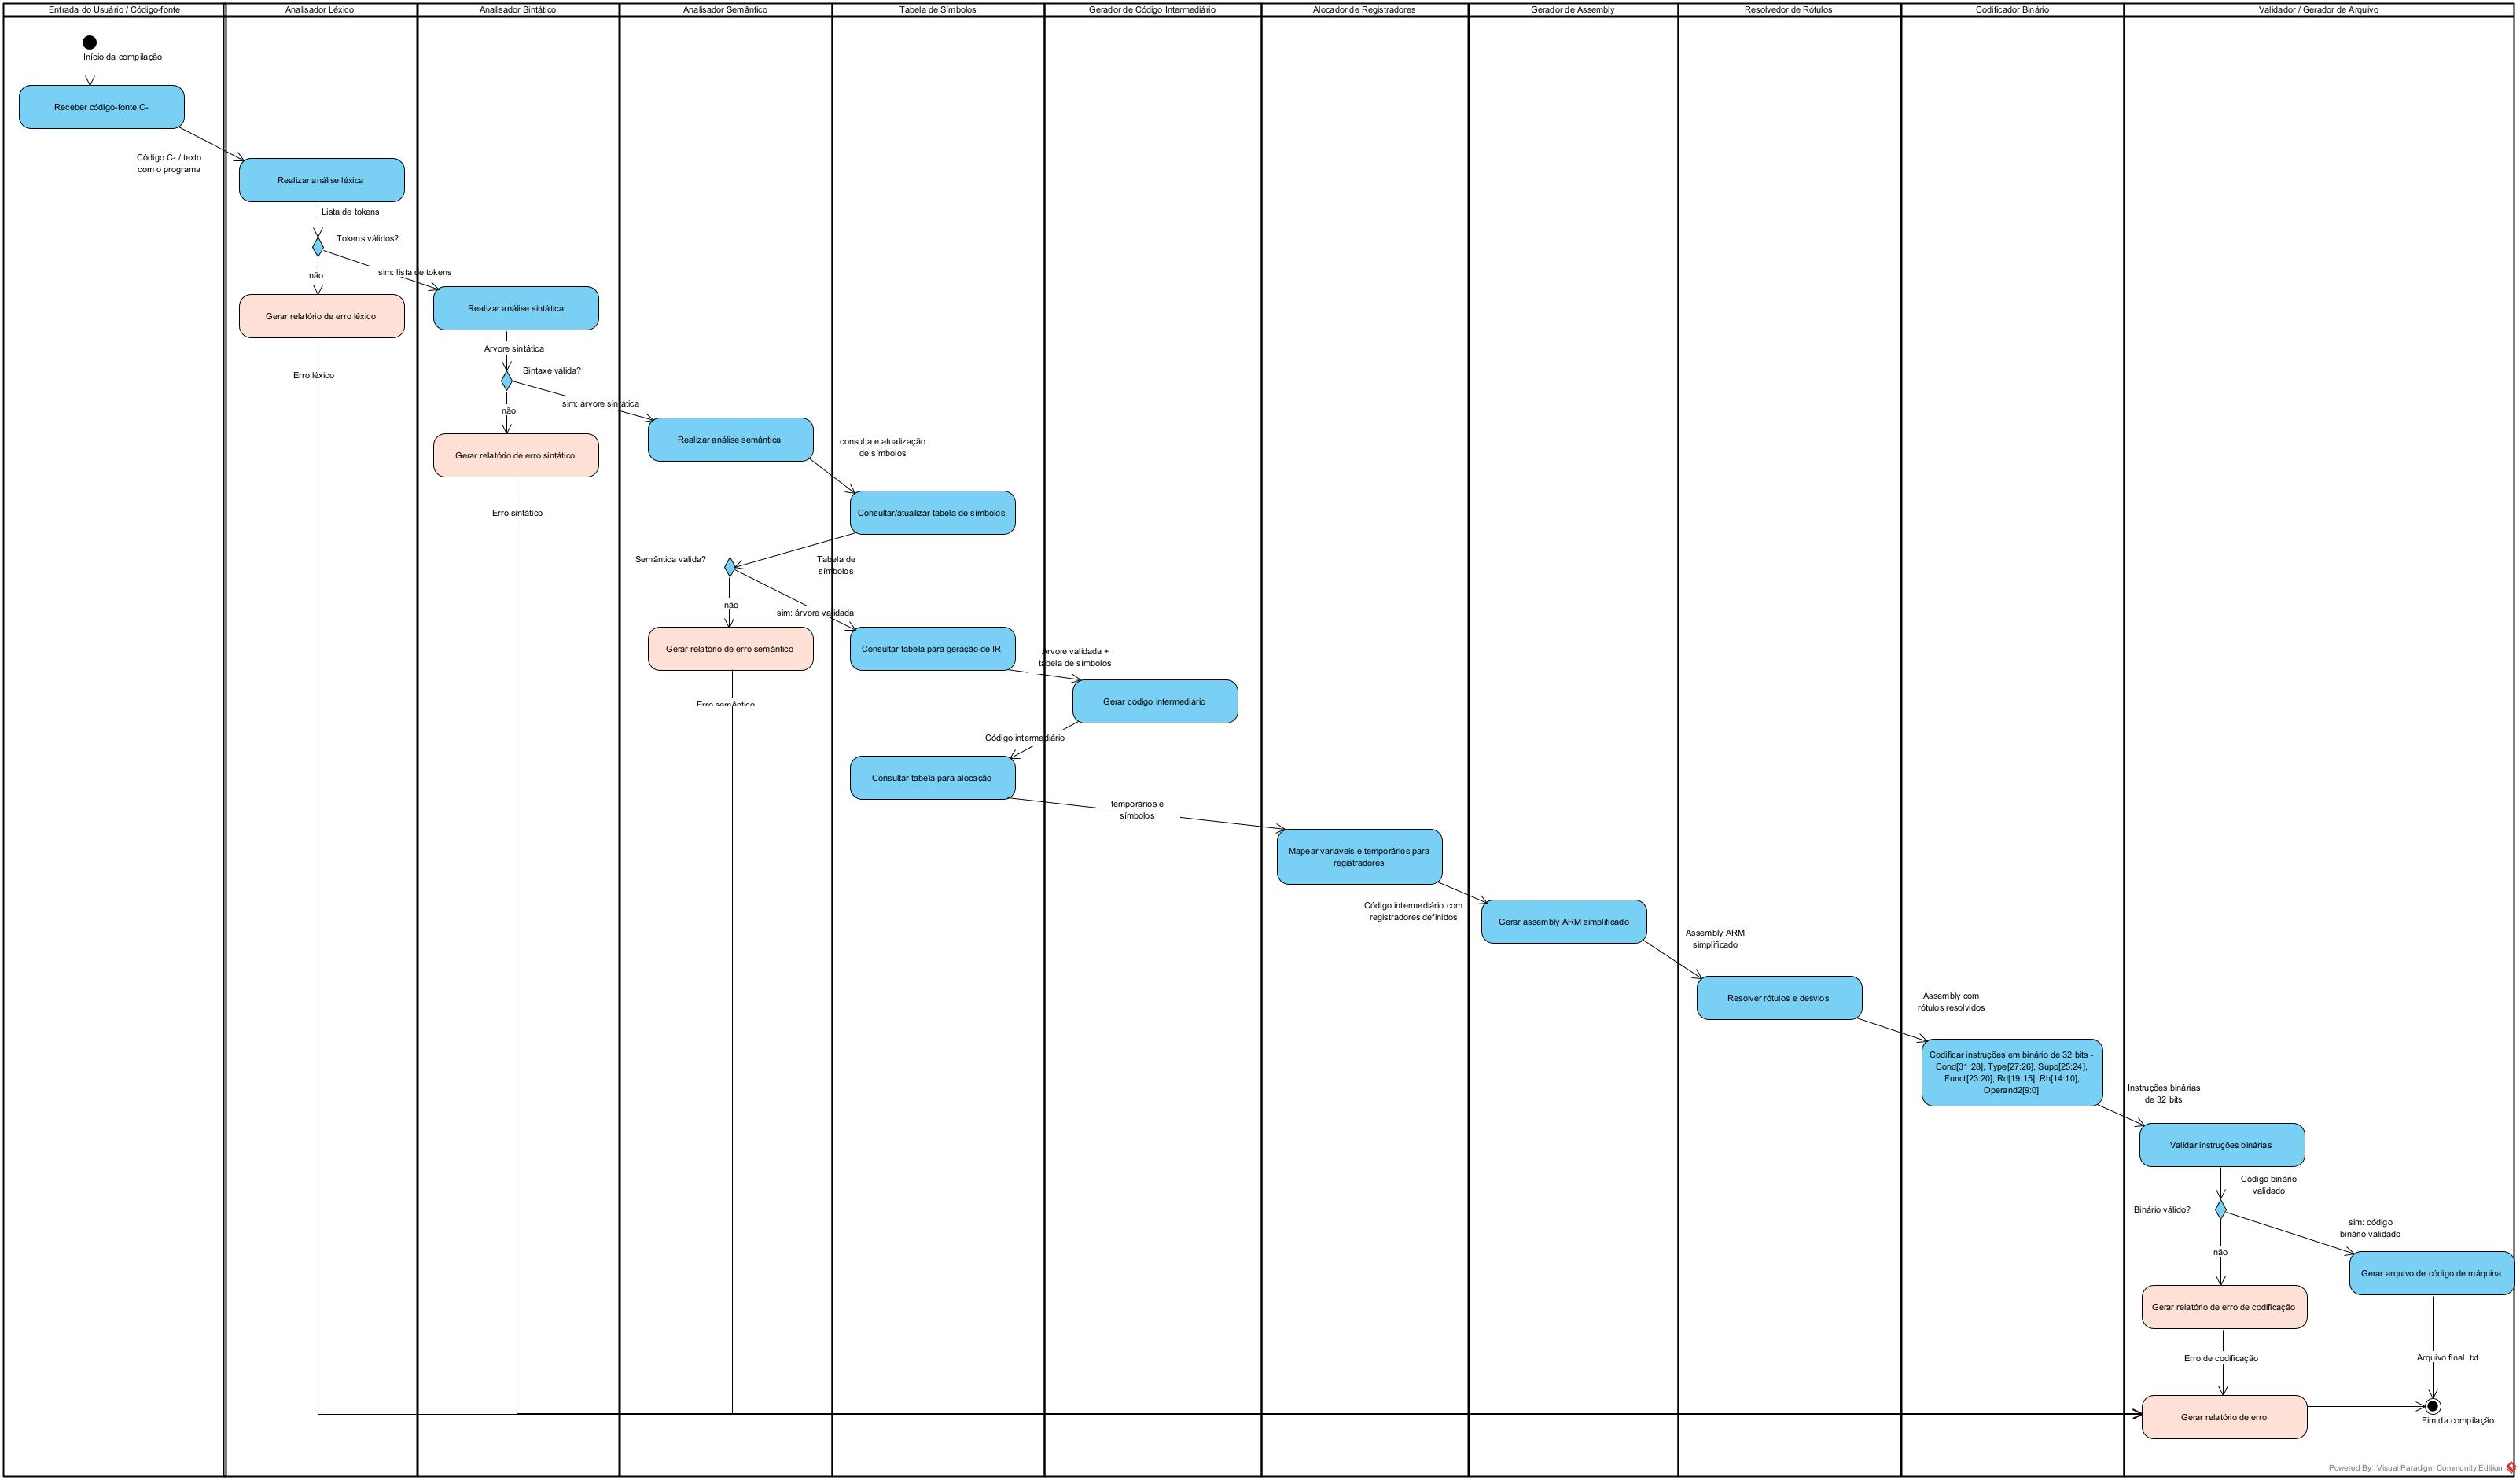
\includegraphics[width=0.7\textwidth]{Diagrama de Atividades - Fluxo de Compilação C- para Código Binário ARM Simplificado.jpg}
    \legend{Fonte: O autor.}
\end{figure}

\begin{figure}[H]
    \centering
    \caption{Diagrama de Blocos da Análise Sintática}
    \graphicspath{ {./Imagens/} }
    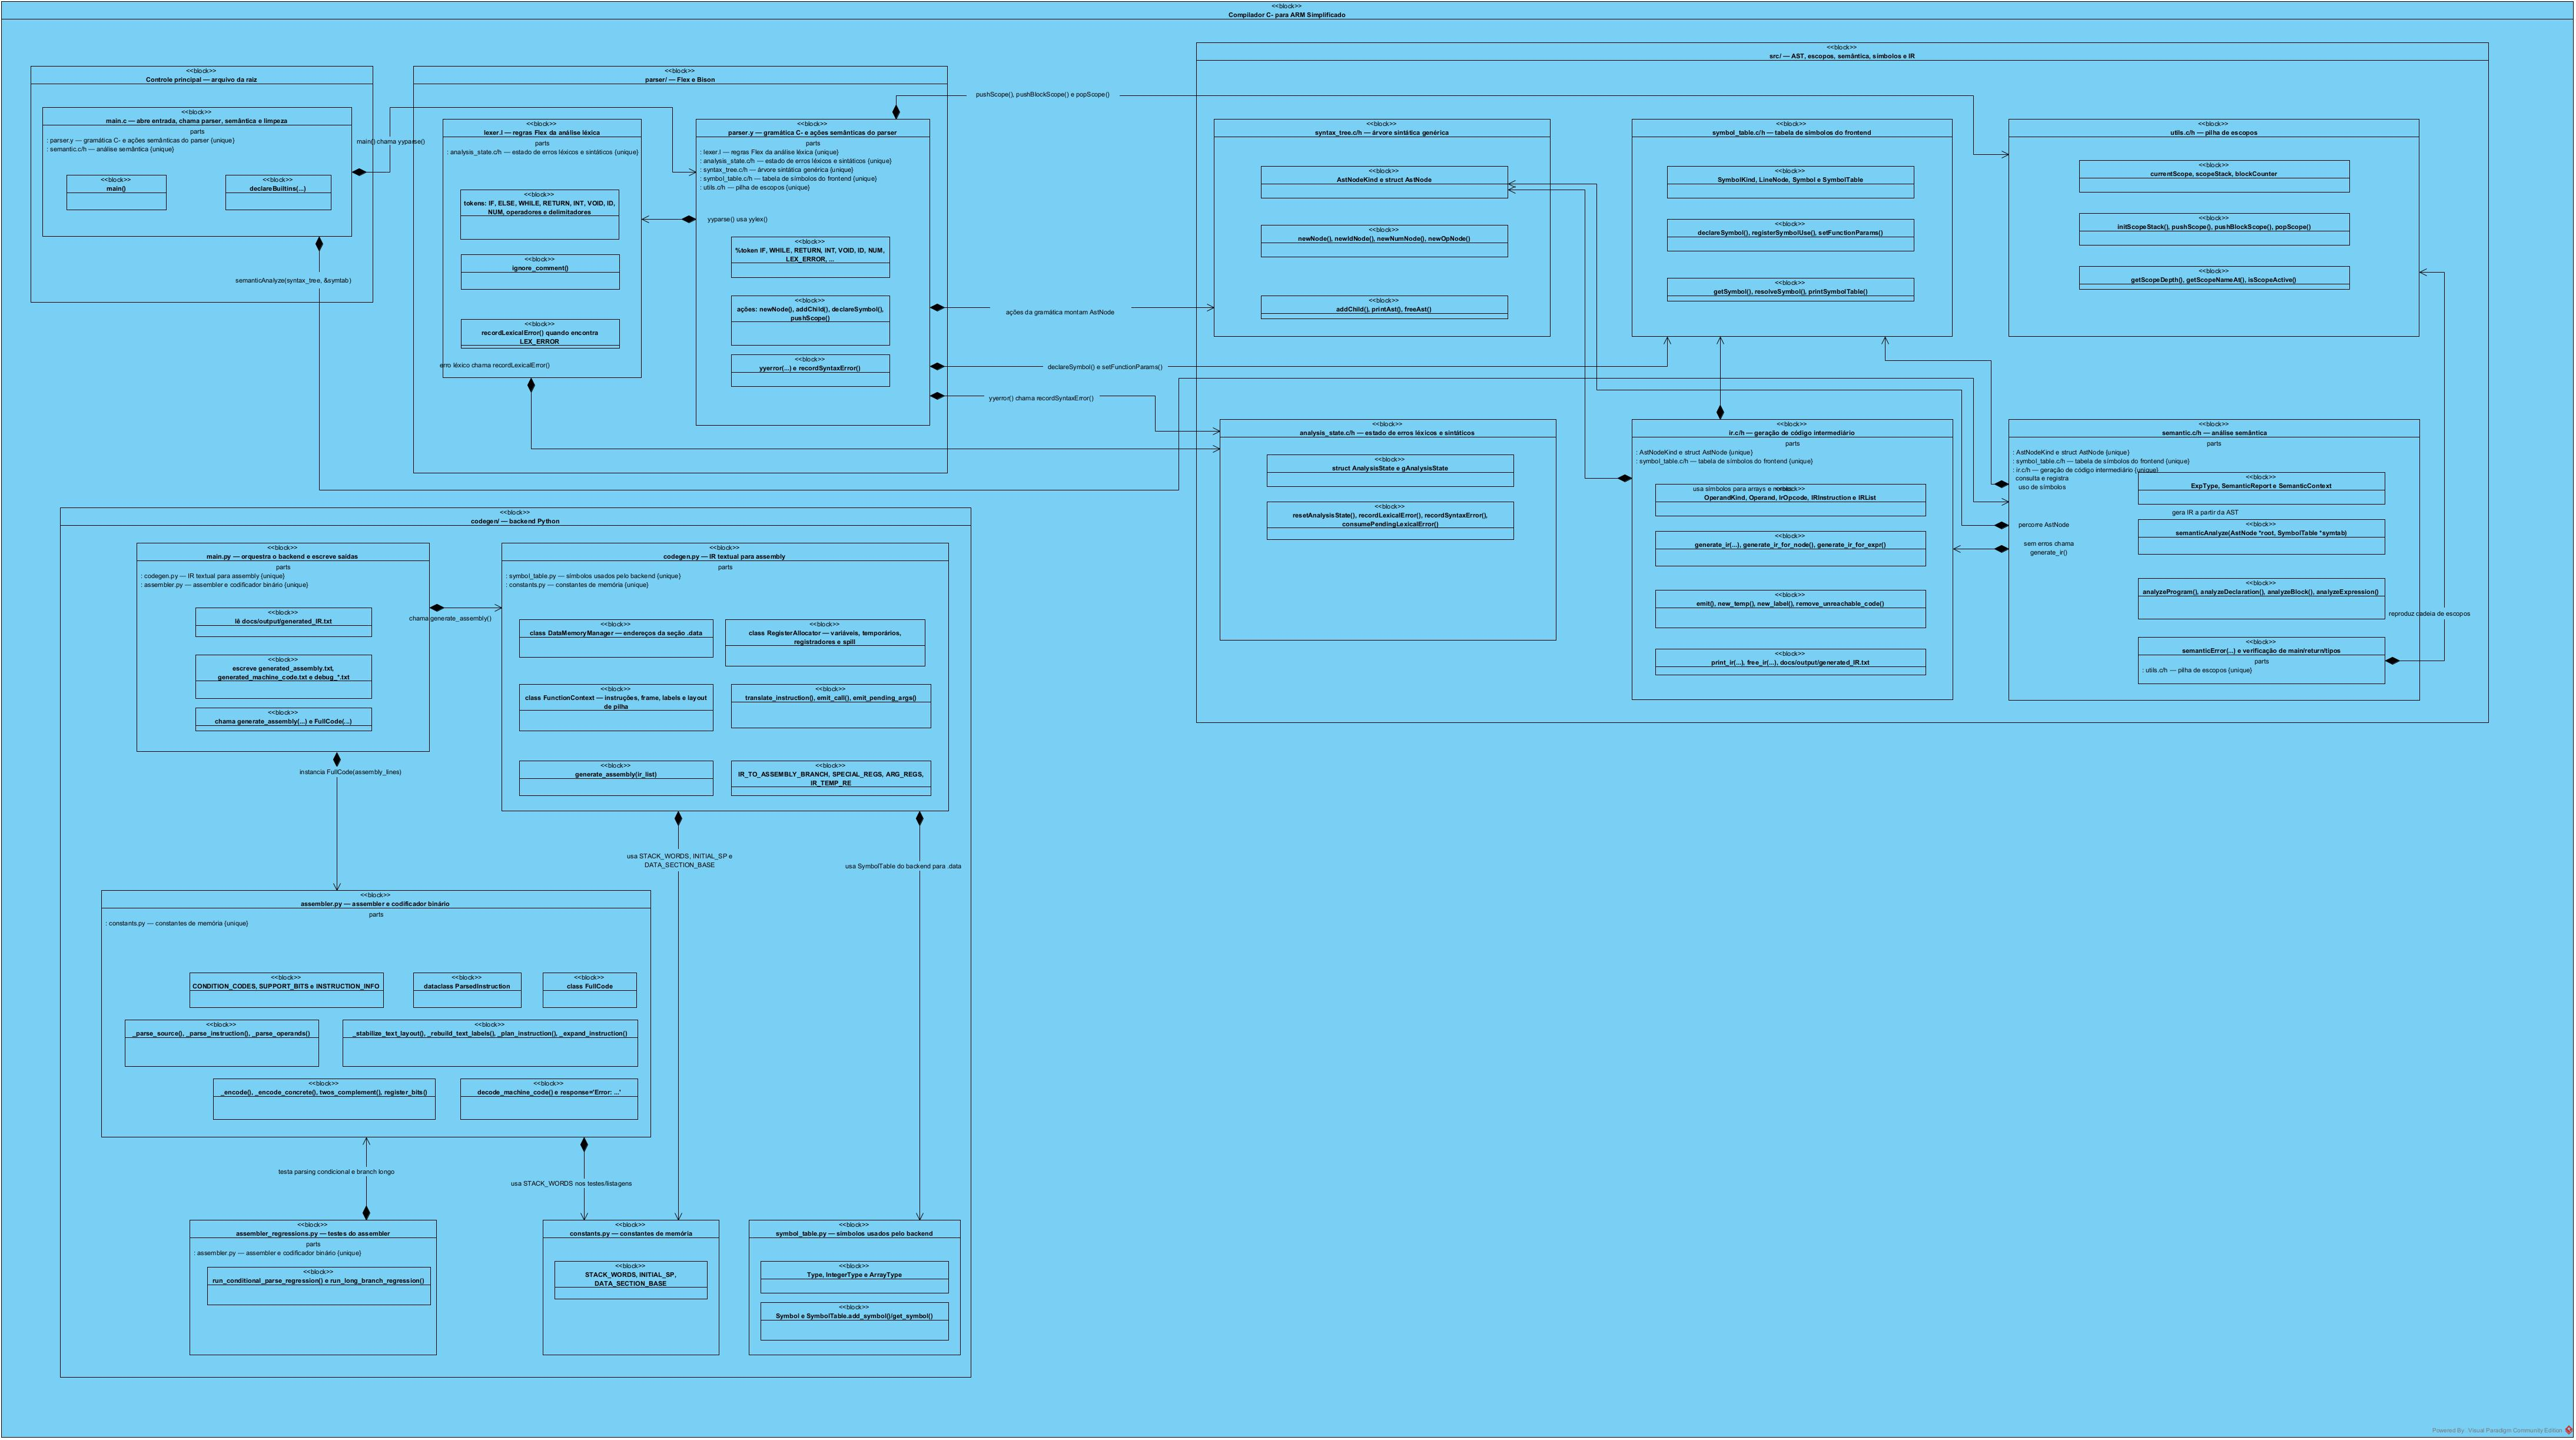
\includegraphics[width=0.8\textwidth]{Diagrama de Blocos — Hierarquia dos Módulos do Compilador.jpg}
    \legend{Fonte: O autor.}
\end{figure}

\begin{figure}[H]
    \centering
    \caption{Diagrama de Atividades da Análise Sintática}
    \graphicspath{ {./Imagens/} }
    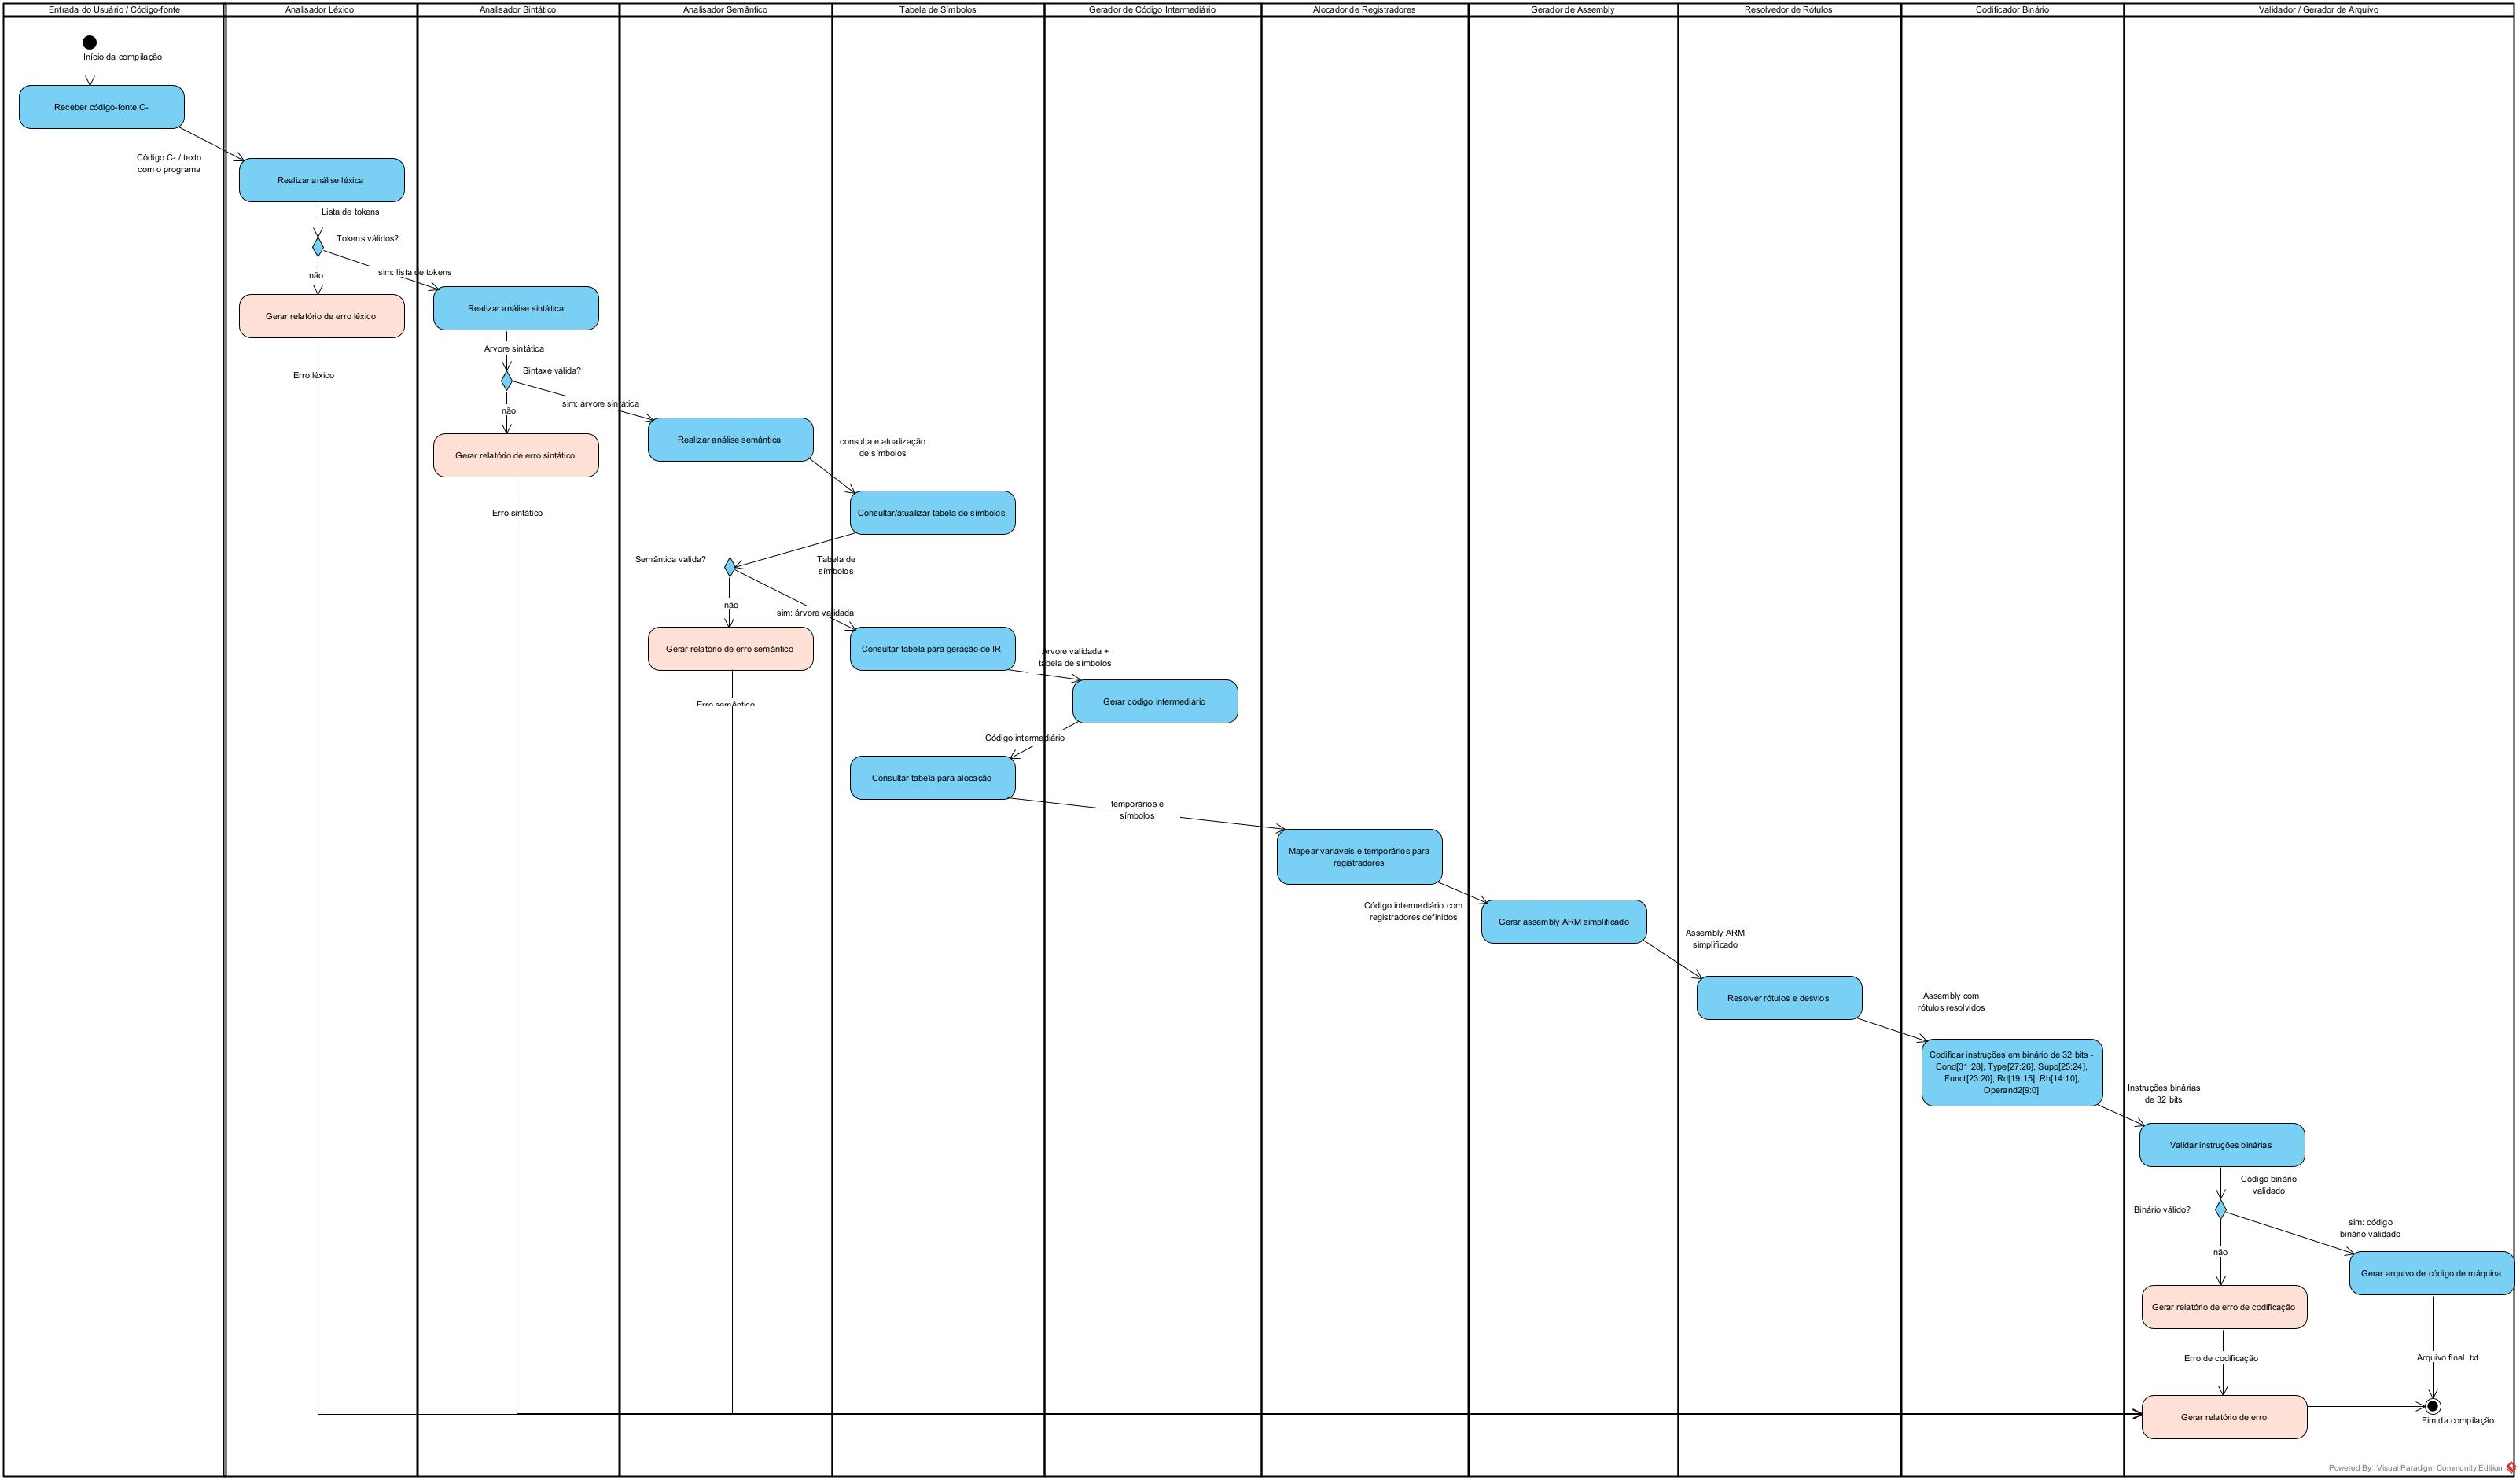
\includegraphics[width=0.7\textwidth]{Diagrama de Atividades - Fluxo de Compilação C- para Código Binário ARM Simplificado.jpg}
    \legend{Fonte: O autor.}
\end{figure}

\begin{figure}[H]
    \centering
    \caption{Diagrama de Blocos da Análise Semântica}
    \graphicspath{ {./Imagens/} }
    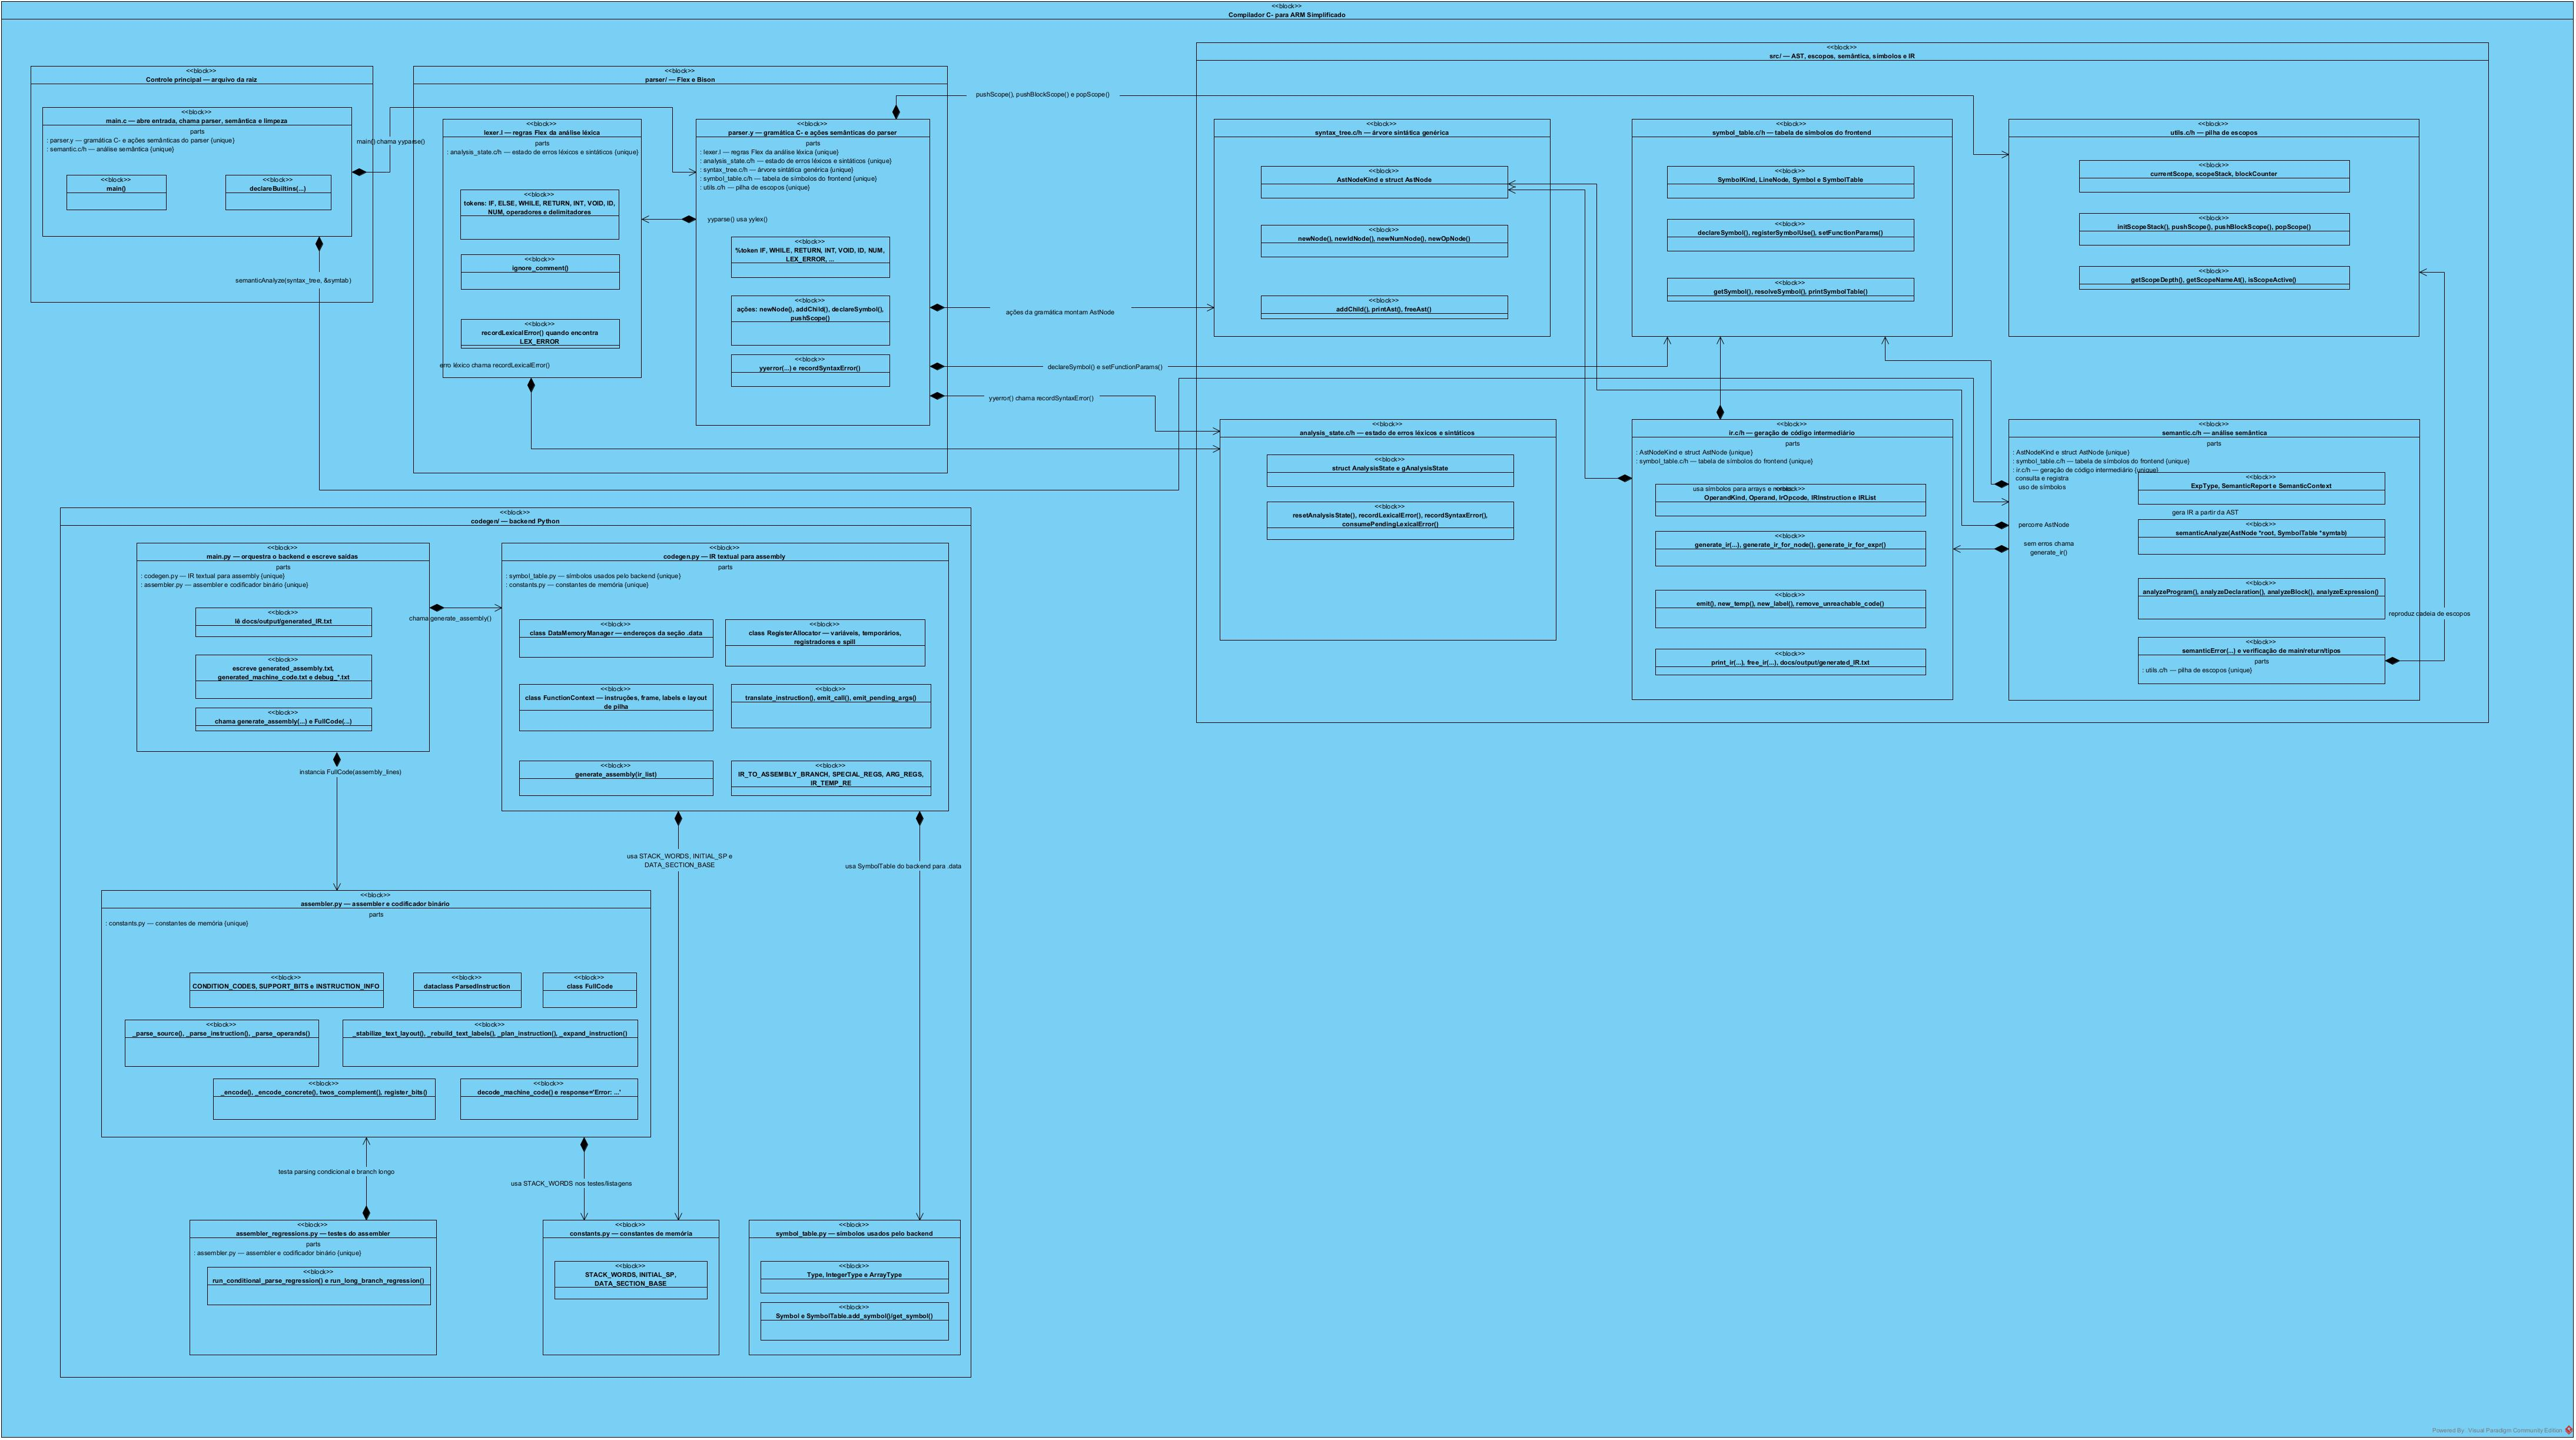
\includegraphics[width=\textwidth]{Diagrama de Blocos — Hierarquia dos Módulos do Compilador.jpg}
    \legend{Fonte: O autor.}
\end{figure}

\begin{figure}[H]
    \centering
    \caption{Diagrama de Atividades da Análise Semântica}
    \graphicspath{ {./Imagens/} }
    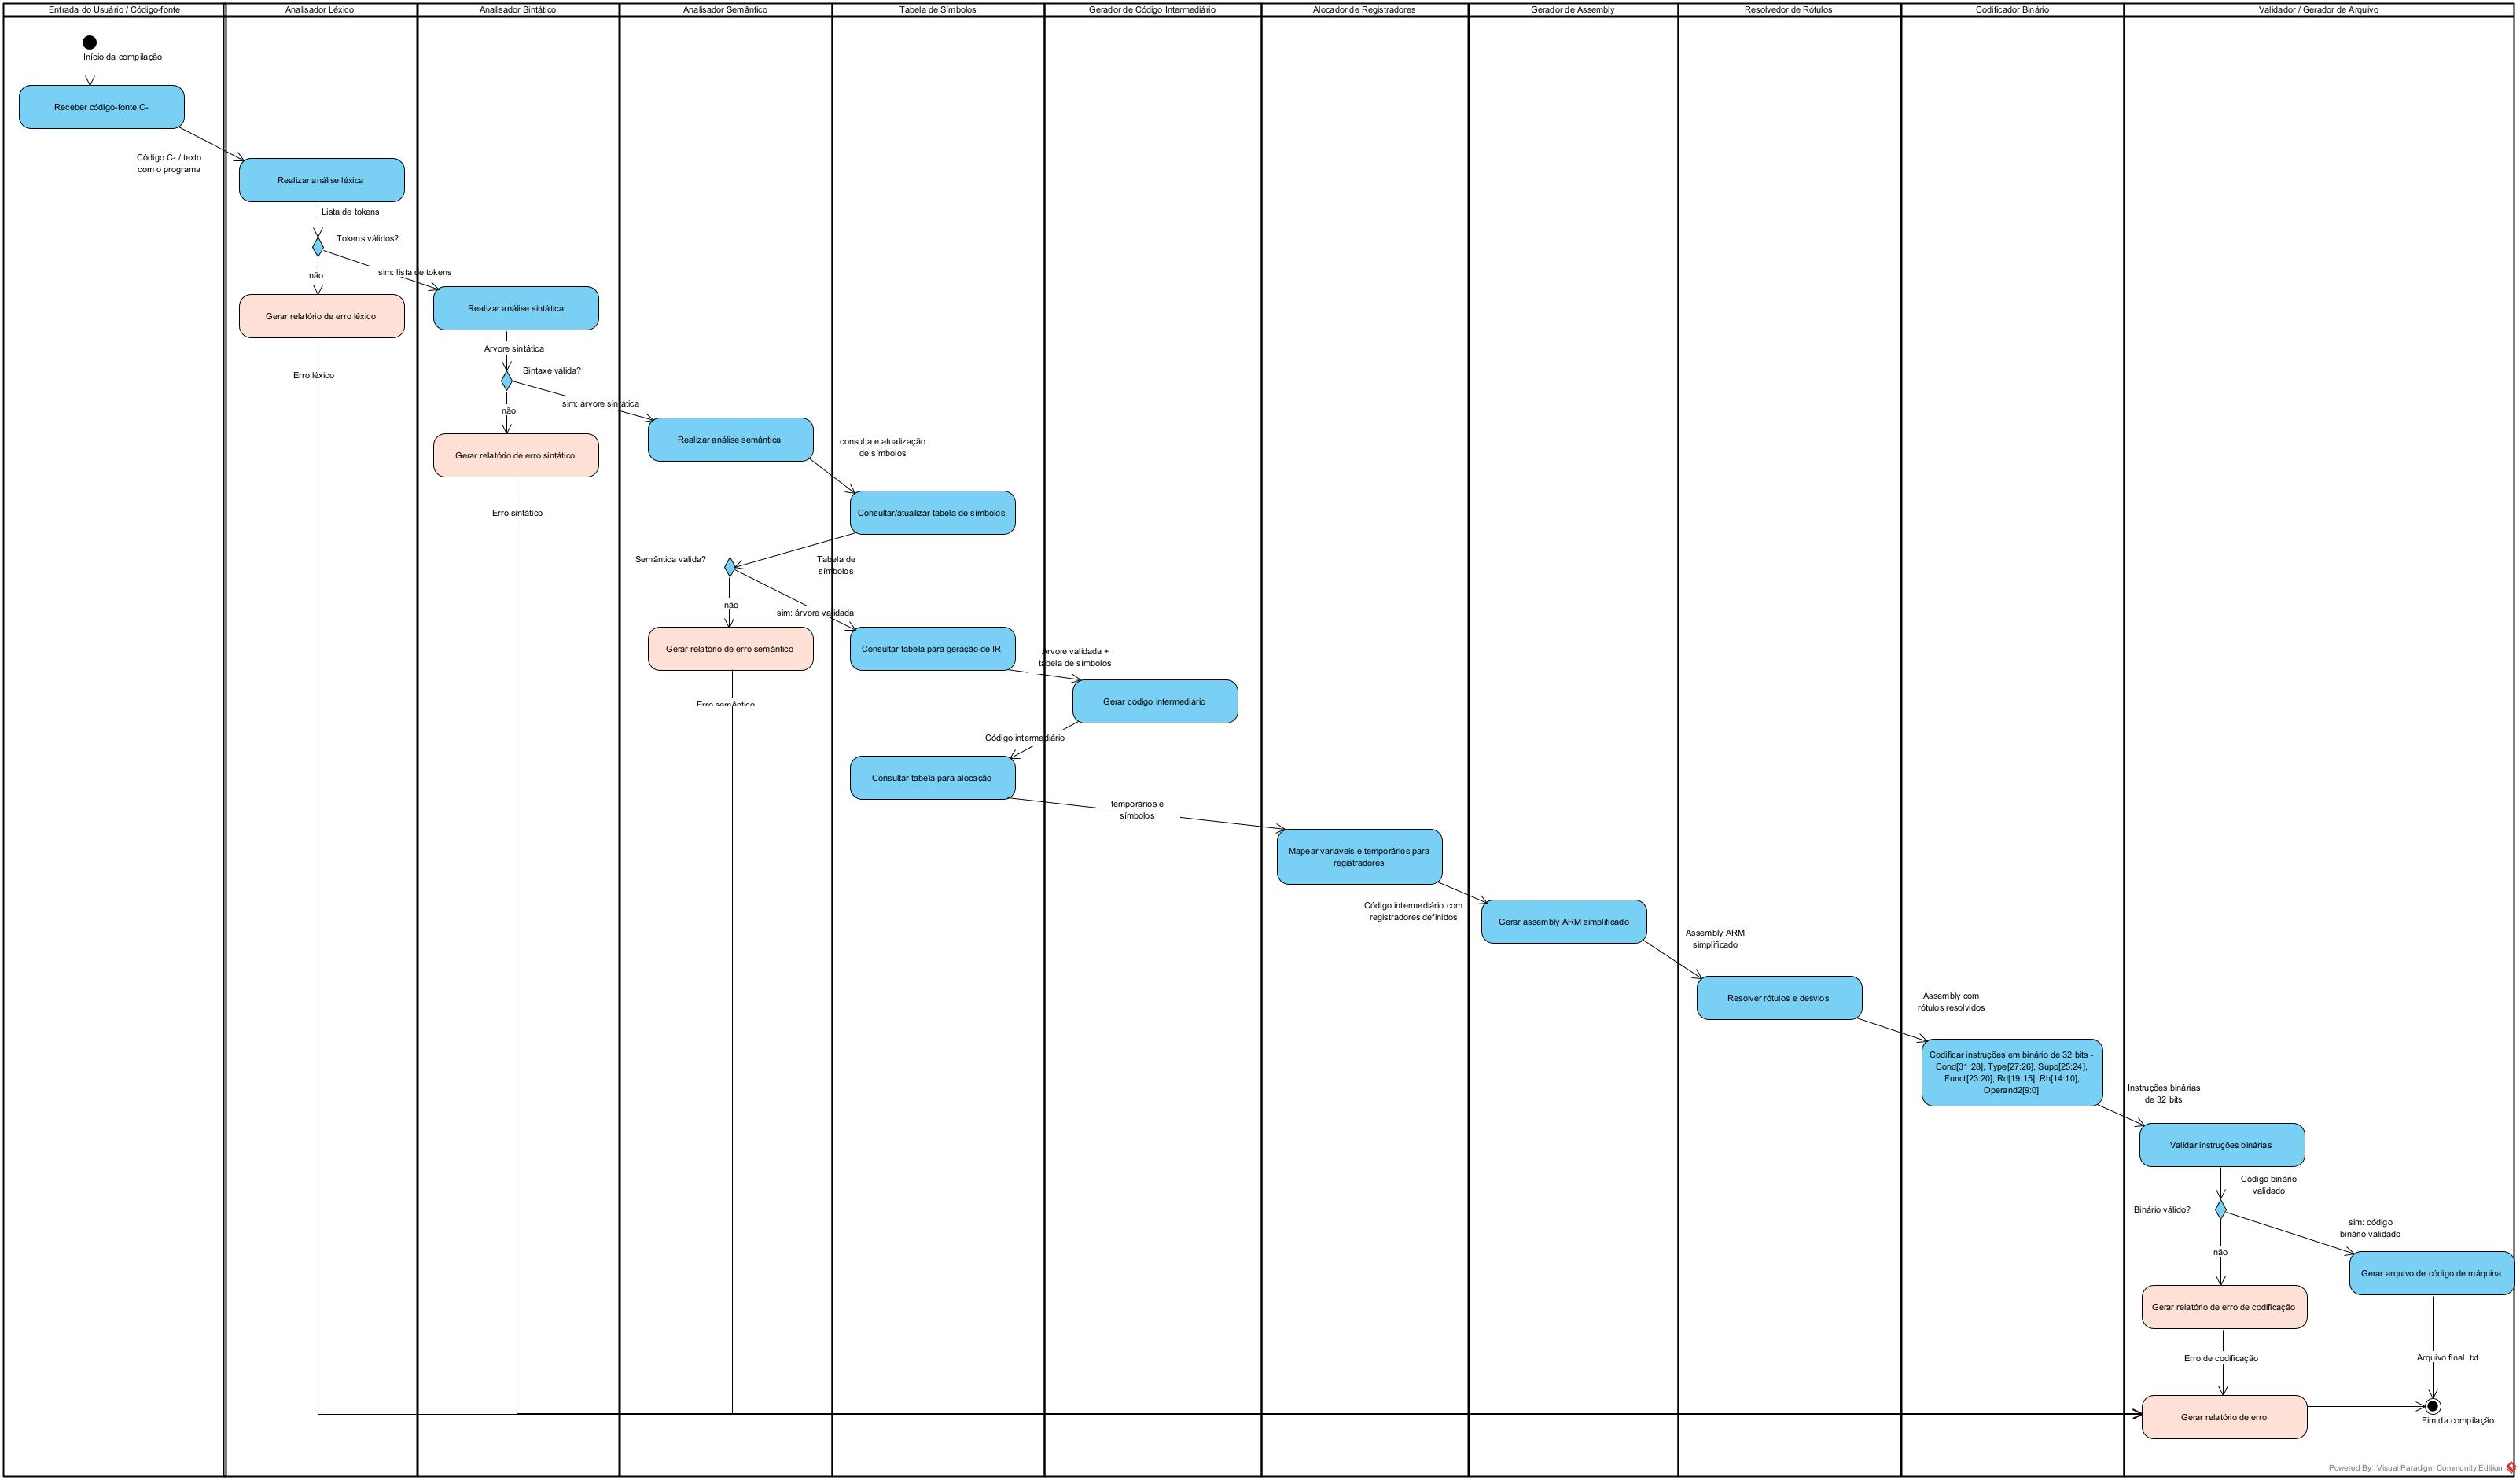
\includegraphics[width=0.9\textwidth]{Diagrama de Atividades - Fluxo de Compilação C- para Código Binário ARM Simplificado.jpg}
    \legend{Fonte: O autor.}
\end{figure}

\newpage
\section{Análise Léxica}

A análise léxica é a primeira etapa do processo de compilação, realizada pelo arquivo \texttt{lexer.l} utilizando a ferramenta Flex. Sua função é ler o fluxo de caracteres do código-fonte e agrupá-los em uma sequência de tokens. Cada token representa uma unidade gramatical, como palavras-chave, identificadores, números e símbolos especiais. Comentários e espaços em branco são identificados e descartados \cite{compiladoresLouden}.

As expressões regulares definidas em \texttt{lexer.l} reconhecem os seguintes padrões:
\begin{itemize}
    \item \textbf{Palavras-chave:} \texttt{if}, \texttt{else}, \texttt{while}, \texttt{return}, \texttt{int}, \texttt{void}.
    \item \textbf{Operadores e Pontuação:} \texttt{==}, \texttt{!=}, \texttt{<=}, \texttt{<}, \texttt{>=}, \texttt{>}, \texttt{=}, \texttt{+}, \texttt{-}, \texttt{*}, \texttt{/}, \texttt{\%}, \texttt{;}, \texttt{,}, \texttt{(}, \texttt{)}, \texttt{\{}, \texttt{\}}, \texttt{[}, \texttt{]}.
    \item \textbf{Identificadores (ID):} Reconhecidos pelo padrão \texttt{[a-zA-Z\_][a-zA-Z0-9\_]*}.
    \item \textbf{Números (NUM):} Reconhecidos pelo padrão \texttt{[0-9]+}.
    \item \textbf{Comentários:} O padrão \texttt{/* ... */} é tratado pela função \texttt{ignore\_comment()}, que consome os caracteres até encontrar o fechamento do comentário.
\end{itemize}
Quando um padrão é reconhecido, o analisador léxico retorna o token correspondente para o analisador sintático, que dará continuidade ao processo.

\section{Análise Sintática}

A análise sintática, ou \emph{parsing}, é implementada no arquivo \texttt{parser.y} com o auxílio da ferramenta Bison. Esta etapa recebe a sequência de tokens do analisador léxico e verifica se eles formam uma estrutura gramatical válida, de acordo com as regras da linguagem C-. O resultado principal desta fase é a construção de uma Árvore Sintática Abstrata (AST), que representa a estrutura hierárquica do código \cite{compiladoresLouden}.

O parser define a gramática livre de contexto da linguagem. Durante a análise, ele empilha os tokens e, ao encontrar uma sequência que corresponde a uma regra gramatical, realiza uma "redução", executando uma ação em C associada. Essas ações são responsáveis por criar os nós da AST (utilizando funções como \texttt{newNode}, \texttt{newIdNode} e \texttt{newOpNode}) e conectá-los (com \texttt{addChild}), formando a árvore que será utilizada nas fases seguintes. Além disso, as ações invocam \texttt{declareSymbol} e \texttt{setFunctionParams} para registrar declarações e assinaturas. O uso efetivo dos símbolos é registrado depois, durante a análise semântica, por meio de \texttt{resolveSymbol} e \texttt{registerSymbolUse}.

Uma diferença importante da versão atual é o tratamento de blocos aninhados. Cada \texttt{compound\_stmt} recebe um nome interno de escopo, gerado por \texttt{pushBlockScope()}, e esse nome é preservado no nó \texttt{AST\_BLOCK}. Dessa forma, a análise semântica e a geração de IR conseguem reconstruir a mesma cadeia de escopos observada pelo parser.

\subsection{Gramática da Linguagem C-}
A seguir, é apresentada uma representação simplificada da gramática implementada no arquivo \texttt{parser.y}, que define a estrutura de um programa válido.

\begin{itemize}
    \item \texttt{program} $\rightarrow$ \texttt{declaration\_list}
    \item \texttt{declaration\_list} $\rightarrow$ \texttt{declaration\_list declaration} | \texttt{declaration}
    \item \texttt{declaration} $\rightarrow$ \texttt{var\_declaration} | \texttt{fun\_declaration}
    \item \texttt{var\_declaration} $\rightarrow$ \texttt{type\_specifier ID ;} | \texttt{type\_specifier ID [ NUM ] ;}
    \item \texttt{fun\_declaration} $\rightarrow$ \texttt{type\_specifier ID ( params ) compound\_stmt}
    \item \texttt{params} $\rightarrow$ \texttt{param\_list} | \texttt{VOID}
    \item \texttt{param\_list} $\rightarrow$ \texttt{param\_list , param} | \texttt{param}
    \item \texttt{param} $\rightarrow$ \texttt{type\_specifier ID} | \texttt{type\_specifier ID [ ]}
    \item \texttt{compound\_stmt} $\rightarrow$ \texttt{\{ local\_declarations statement\_list \}}
    \item \texttt{statement} $\rightarrow$ \texttt{expression\_stmt} | \texttt{compound\_stmt} | \texttt{selection\_stmt} | \texttt{iteration\_stmt} | \texttt{return\_stmt}
    \item \texttt{selection\_stmt} $\rightarrow$ \texttt{IF ( expression ) statement} | \texttt{IF ( expression ) statement ELSE statement}
    \item \texttt{iteration\_stmt} $\rightarrow$ \texttt{WHILE ( expression ) statement}
    \item \texttt{return\_stmt} $\rightarrow$ \texttt{RETURN ;} | \texttt{RETURN expression ;}
    \item \texttt{expression} $\rightarrow$ \texttt{var = expression} | \texttt{simple\_expression}
    \item \texttt{simple\_expression} $\rightarrow$ \texttt{additive\_expression relop additive\_expression} | \texttt{additive\_expression}
    \item \texttt{additive\_expression} $\rightarrow$ \texttt{additive\_expression addop term} | \texttt{term}
    \item \texttt{term} $\rightarrow$ \texttt{term mulop factor} | \texttt{factor}
    \item \texttt{factor} $\rightarrow$ \texttt{( expression )} | \texttt{var} | \texttt{call} | \texttt{NUM}
    \item \texttt{call} $\rightarrow$ \texttt{ID ( args )}
\end{itemize}

\section{Análise Semântica}

A análise semântica é a fase que verifica o significado do código e garante sua coerência, indo além da simples verificação estrutural da sintaxe. A implementação utiliza a AST gerada na fase anterior e uma Tabela de Símbolos para realizar as validações \cite{compiladoresLouden}. As principais verificações incluem:
\begin{itemize}
    \item \textbf{Declaração de Variáveis e Funções:} Garante que todos os identificadores sejam declarados antes do uso.
    \item \textbf{Verificação de Tipos:} Assegura que os tipos em atribuições, operações e retornos de função sejam compatíveis.
    \item \textbf{Escopo:} Controla a visibilidade de variáveis, diferenciando entre escopo global, escopo de função e blocos aninhados.
    \item \textbf{Unicidade:} Impede a redeclaração de variáveis ou funções no mesmo escopo.
    \item \textbf{Chamadas de Função:} Verifica se as funções são chamadas com o número correto de argumentos.
\end{itemize}

A Tabela de Símbolos, gerenciada pelas funções em \texttt{symbol\_table.h}, armazena informações sobre cada identificador, como seu nome, tipo, escopo e linha de declaração, sendo fundamental para todas essas verificações.

\begin{table}[H]
    \centering
    \ABNTEXfontereduzida
    \caption{Matriz de verificações semânticas implementadas}
    \label{tab:matriz_semantica}
    \begin{tabular}{|p{0.26\textwidth}|p{0.33\textwidth}|p{0.27\textwidth}|}
        \hline
        \textbf{Verificação} & \textbf{Funções envolvidas} & \textbf{Efeito esperado} \\
        \hline
        Identificador não declarado & \texttt{resolveSymbol}, \texttt{analyzeExpression} & Emite erro semântico e impede geração de IR. \\
        \hline
        Redeclaração no mesmo escopo & \texttt{hasEarlierDeclaration}, \texttt{analyzeVariableDeclaration}, \texttt{analyzeFunctionDeclaration} & Rejeita símbolos repetidos no mesmo escopo, mas permite sombreamento em blocos diferentes. \\
        \hline
        Uso incorreto de vetor & \texttt{analyzeArrayAccess}, \texttt{analyzeAssignmentTarget} & Impede atribuição ao vetor inteiro e exige índice inteiro. \\
        \hline
        Chamada de função & \texttt{getParamCount}, \texttt{getParamType}, \texttt{analyzeExpression} & Confere quantidade e tipos dos argumentos. \\
        \hline
        Retorno de função & \texttt{statementGuaranteesReturn}, \texttt{blockGuaranteesReturn} & Rejeita função \texttt{int} sem retorno em todos os caminhos estruturais. \\
        \hline
        Função principal & \texttt{hasMainFunction} & Exige função global \texttt{main}. \\
        \hline
    \end{tabular}
    \legend{Fonte: O autor.}
\end{table}

Somente quando essas verificações terminam sem erros o compilador chama \texttt{generate\_ir}. Essa decisão evita que o back-end tente traduzir programas estruturalmente válidos, mas semanticamente indefinidos.

%------------------- Fase de Síntese -------------------
\chapter{Compilador: Fase de Síntese}
\label{cap:sintese}

No sistema integrado, a fase de síntese é o ponto em que as decisões do compilador encontram as restrições reais do processador. Ela traduz a representação intermediária do programa para o código de máquina da arquitetura alvo, respeitando a quantidade de registradores, o formato das instruções, a RAM de 64 palavras e as regras de desvio do \texttt{Processor(v2026-1)}. No projeto atual, a IR ainda é gerada no front-end em C, pelo gerador de IR, e o back-end propriamente dito é implementado em Python. Essa separação cria um contrato simples entre as linguagens: o C grava o arquivo de IR gerado; o Python lê esse arquivo, gera o assembly intermediário e depois o converte para o código de máquina final de 32 bits.

\begin{table}[H]
    \centering
    \ABNTEXfontereduzida
    \caption{Agrupamento dos módulos da fase de síntese}
    \label{tab:modulos_sintese}
    \begin{tabular}{|p{0.24\textwidth}|p{0.27\textwidth}|p{0.35\textwidth}|}
        \hline
        \textbf{Grupo} & \textbf{Arquivos} & \textbf{Responsabilidade} \\
        \hline
        IR & \texttt{ir.c/h} & Lineariza a AST em código de três endereços com temporários, rótulos, declarações globais e remoção de código inalcançável. \\
        \hline
        Geração de assembly & \texttt{codegen.py} & Calcula frames, aloca registradores com \texttt{RegisterAllocator}, traduz IR e emite prólogo/epílogo. \\
        \hline
        Símbolos do back-end & \texttt{symbol\_table.py} & Representa variáveis globais, inteiros, vetores e endereços de dados. \\
        \hline
        Constantes de memória & \texttt{constants.py} & Define pilha de 64 palavras, \texttt{sp} inicial 63 e base conceitual de dados 64. \\
        \hline
        Montador & \texttt{assembler.py} & Resolve rótulos, expande literais, expande branches longos e codifica instruções de 32 bits. \\
        \hline
        Execução simulada & Simulador de código de máquina & Executa o binário contra um modelo Python do \texttt{Processor(v2026-1)}. \\
        \hline
    \end{tabular}
    \legend{Fonte: O autor.}
\end{table}

\section{Modelagem}

A modelagem da fase de síntese também foi guiada por diagramas SysML, que ilustram a estrutura e o fluxo de dados desde a Árvore Sintática Abstrata (AST) até o código de máquina final.

\begin{figure}[H]
    \centering
    \caption{Diagrama de Blocos do Gerador de Código}
    \graphicspath{ {./Imagens/} }
    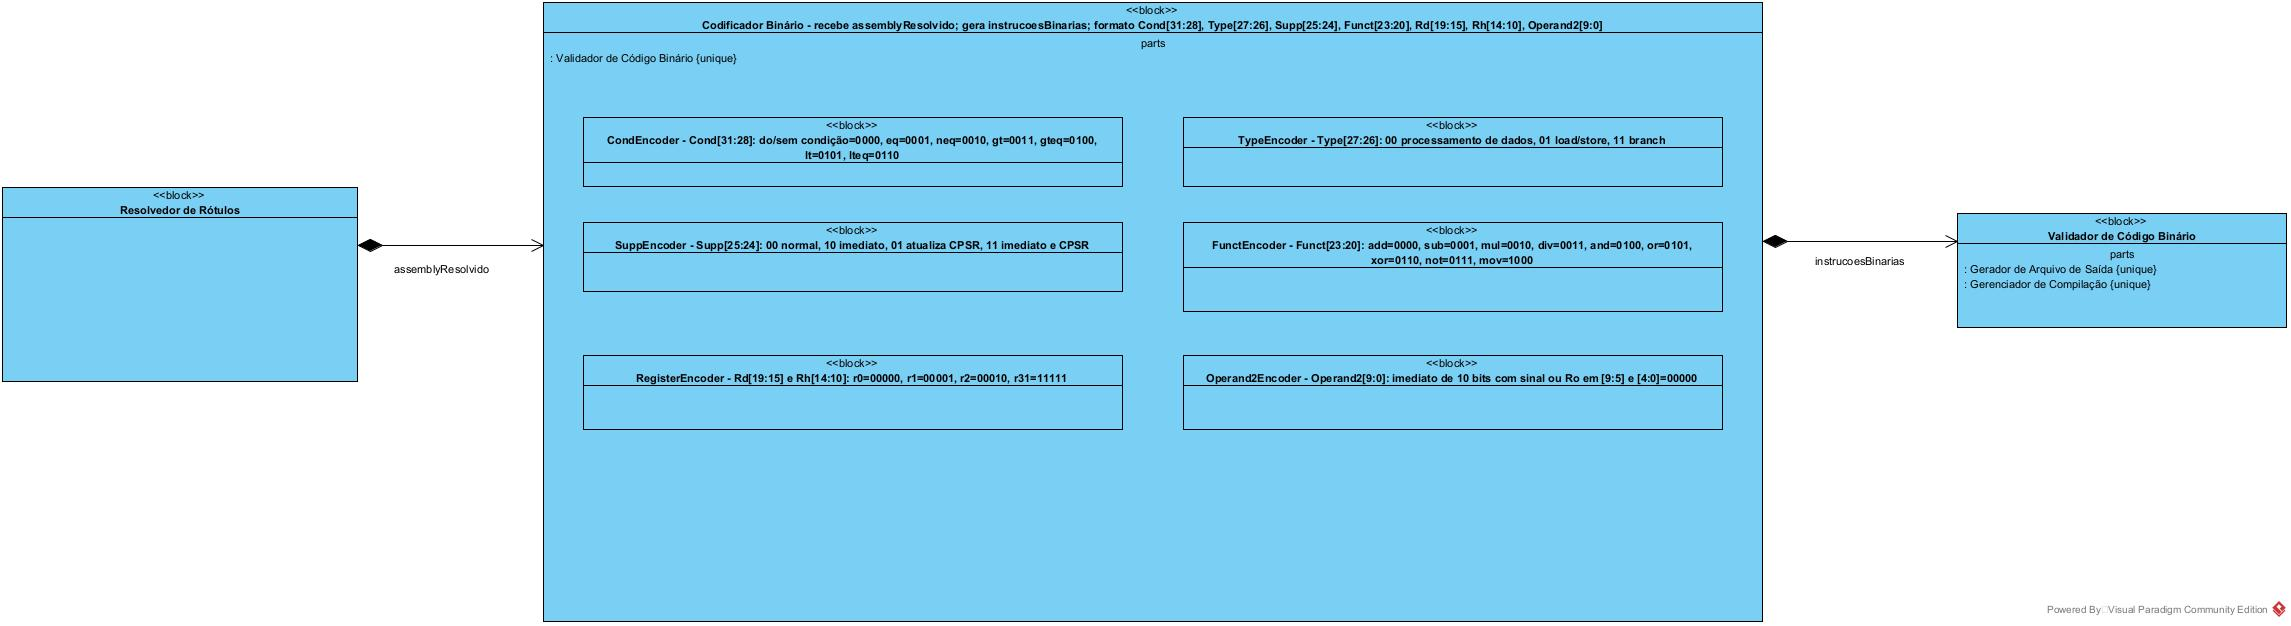
\includegraphics[width=\textwidth]{Diagrama Interno - Codificador Binário.jpg}
    \legend{Fonte: O autor.}
\end{figure}

\begin{figure}[H]
    \centering
    \caption{Diagrama de Atividades do Gerador de Código}
    \graphicspath{ {./Imagens/} }
    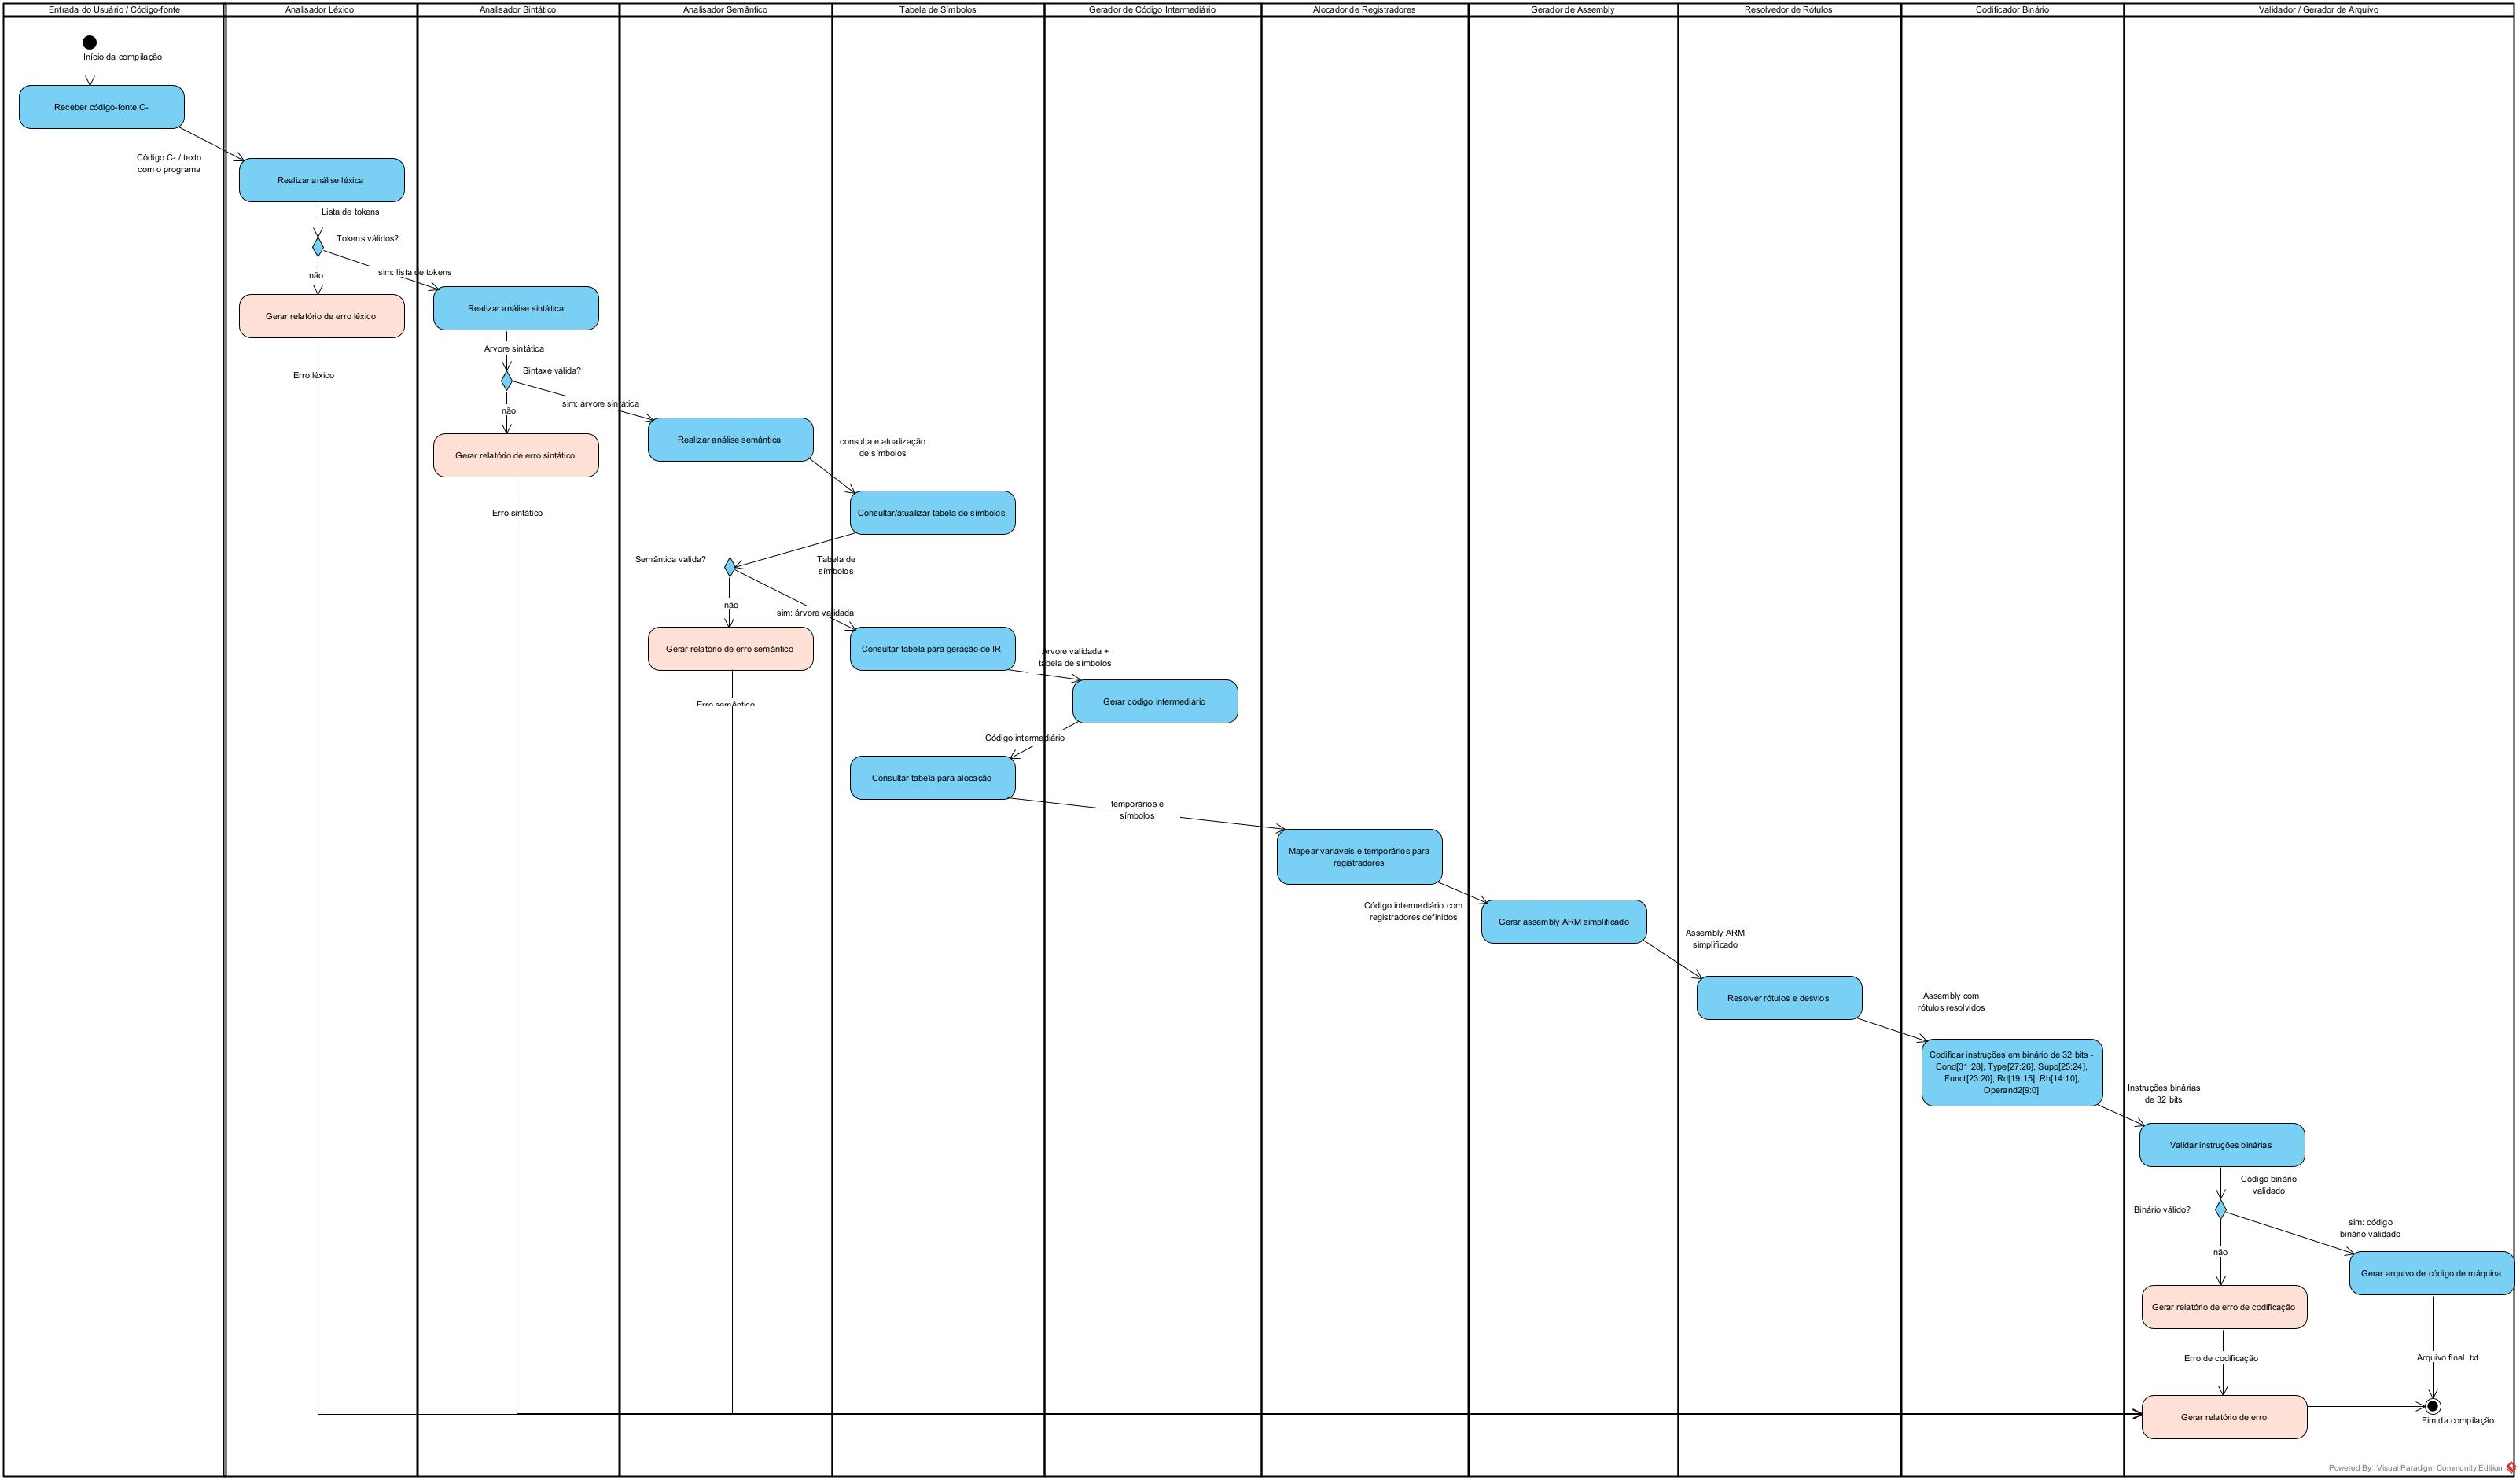
\includegraphics[width=0.4\textwidth]{Diagrama de Atividades - Fluxo de Compilação C- para Código Binário ARM Simplificado.jpg}
    \legend{Fonte: O autor.}
\end{figure}

\section{Geração do Código Intermediário}

A geração de Código Intermediário (IR) é a última etapa do front-end e a primeira representação consumida pelo back-end. O gerador de IR percorre a AST e gera uma representação linear, no formato de código de três endereços \cite{compiladoresLouden}. Essa forma é menos dependente da árvore sintática e mais adequada para tradução para assembly. As operações do IR, definidas em \texttt{ir.h}, são detalhadas na \autoref{tab:ir_opcodes}.

A função \texttt{generate\_ir} coordena essa etapa, reinicializando contadores, chamando \texttt{generate\_global\_declarations}, percorrendo a AST com \texttt{generate\_ir\_for\_node} e delegando expressões para \texttt{generate\_ir\_for\_expr}. A emissão das instruções é centralizada em \texttt{emit}; temporários e rótulos são produzidos por \texttt{new\_temp} e \texttt{new\_label}. Ao final, \texttt{remove\_unreachable\_code} elimina trechos inalcançáveis após desvios e retornos, e \texttt{print\_ir} grava o arquivo de IR gerado.

\begin{table}[H]
    \centering
    \ABNTEXfontereduzida
    \caption{Definição das Operações do Código Intermediário (IR)}
    \label{tab:ir_opcodes}
    \begin{tabular}{|l|l|}
        \hline
        \textbf{Opcode (IR)} & \textbf{Função e Formato} \\
        \hline \hline
        \texttt{IR\_ASSIGN} & Atribuição simples: \texttt{resultado := arg1} \\
        \hline
        \texttt{IR\_LOAD} & Carrega valor da memória: \texttt{resultado := *arg1} \\
        \hline
        \texttt{IR\_STORE} & Armazena valor na memória: \texttt{*resultado := arg1} \\
        \hline
        \texttt{IR\_ADDR} & Obtém endereço de uma variável: \texttt{resultado := \&arg1} \\
        \hline
        \texttt{IR\_DEC} & Declara espaço de dados: \texttt{resultado := .word/.space, tamanho} \\
        \hline
        \texttt{IR\_ADD / SUB / MUL / DIV} & Operações aritméticas: \texttt{resultado := arg1 op arg2} \\
        \hline
        \texttt{IR\_EQ / NEQ / LT / LTE / GT / GTE} & Operações de comparação: \texttt{resultado := (arg1 op arg2)} \\
        \hline
        \texttt{IR\_LABEL} & Define um rótulo no código: \texttt{resultado:} \\
        \hline
        \texttt{IR\_GOTO} & Desvio incondicional: \texttt{goto resultado} \\
        \hline
        \texttt{IR\_IF\_GOTO} & Desvio condicional: \texttt{if\_false arg1 goto resultado} \\
        \hline
        \texttt{IR\_RETURN} & Retorna de uma função, com ou sem valor: \texttt{return resultado} \\
        \hline
        \texttt{IR\_PARAM} & Registra parâmetro formal no início da função: \texttt{param resultado} \\
        \hline
        \texttt{IR\_ARG} & Define um argumento para uma chamada de função: \texttt{arg resultado} \\
        \hline
        \texttt{IR\_CALL} & Chamada de função com valor de retorno: \\ \texttt{resultado := call arg1, arg2} \\
        \hline
        \texttt{IR\_PCALL} & Chamada de procedimento (sem retorno): \texttt{call resultado, arg1} \\
        \hline
        \texttt{IR\_INOUT\_CALL} & Opcode reservado no cabeçalho para chamadas de entrada/saída; \\
        o fluxo atual usa \texttt{IR\_CALL}/\texttt{IR\_PCALL} para \texttt{input} e \texttt{output}. \\
        \hline
    \end{tabular}
    \legend{Fonte: O autor.}
\end{table}

O operador \texttt{\%}, aceito pela gramática, não possui instrução nativa no processador. Por isso, o IR o reduz para a identidade \texttt{a \% b = a - ((a / b) * b)}. Outra decisão relevante é que os vetores são endereçados por palavra; assim, o índice é somado ao endereço base, sem multiplicação por 4.

\section{Geração do Código Assembly}

O script \texttt{codegen.py} lê o código intermediário e o traduz para a linguagem Assembly do processador alvo, gravando o assembly gerado \cite{compiladoresLouden,compOrgDes}. Esta etapa envolve:
\begin{itemize}
    \item \textbf{Alocação de Registradores:} Um gerenciador de registradores (\texttt{RegisterAllocator}) mapeia as variáveis temporárias e do código-fonte para os registradores físicos do processador. Ele implementa uma estratégia de \emph{spill} para lidar com a escassez de registradores, salvando valores na pilha quando necessário e preservando valores ao redor de chamadas de função.
    \item \textbf{Gerenciamento de Memória:} Um \texttt{DataMemoryManager} aloca espaço na seção \texttt{.data} para variáveis globais e literais.
    \item \textbf{Tradução de Instruções:} Cada operação do IR é mapeada para uma ou mais instruções Assembly, gerenciando o fluxo de controle (\emph{branches}), acesso à memória (\emph{loads/stores}), operações aritméticas, prólogo, epílogo, chamadas de função, recursão e retorno em \texttt{r0}.
\end{itemize}

\begin{table}[H]
    \centering
    \ABNTEXfontereduzida
    \caption{Convenção de registradores usada pelo back-end}
    \label{tab:convencao_registradores}
    \begin{tabular}{|p{0.22\textwidth}|p{0.18\textwidth}|p{0.44\textwidth}|}
        \hline
        \textbf{Nome lógico} & \textbf{Registrador} & \textbf{Uso} \\
        \hline
        Valor de retorno & \texttt{r0} & Guarda o retorno de funções \texttt{int}. \\
        \hline
        Argumentos rápidos & \texttt{r1--r3} & Recebem os três primeiros argumentos de chamada. \\
        \hline
        Temporários preferenciais & \texttt{r4--r11} & Usados para cálculos de curta duração. \\
        \hline
        Registradores preserváveis & \texttt{r12--r26} & Preferidos para valores de maior vida útil. \\
        \hline
        Auxiliar do montador & \texttt{r27} & Usado em expansões de literais e branches longos. \\
        \hline
        Link lógico & \texttt{r28} & Usado pelo assembly como \texttt{lr}; deve ser distinguido do link dedicado do RTL. \\
        \hline
        Ponteiro de pilha & \texttt{r29} & Representa \texttt{sp}. \\
        \hline
        Registrador de spill & \texttt{r30} & Auxilia cargas/armazenamentos durante derramamento. \\
        \hline
        Ponteiro de frame & \texttt{r31} & Representa \texttt{fp}. \\
        \hline
    \end{tabular}
    \legend{Fonte: O autor.}
\end{table}

\section{Geração do Código Executável}

A etapa final é a montagem, realizada pelo \texttt{assembler.py}. Este script realiza um processo de duas passagens:
\begin{enumerate}
    \item \textbf{Análise e mapeamento:} Lê o código Assembly, separa as seções \texttt{.text} e \texttt{.data}, identifica rótulos e constrói uma tabela de símbolos.
    \item \textbf{Estabilização de layout:} Calcula o tamanho efetivo de cada instrução, repetindo a análise quando uma instrução precisa ser expandida. Isso é necessário para \texttt{movi} com imediato fora de 10 bits e para branches que não alcançam o alvo com deslocamento imediato.
    \item \textbf{Codificação final:} Traduz cada instrução concreta para o formato binário de 32 bits, calcula offsets PC-relativos e preserva a correspondência entre instrução simbólica e palavra codificada.
\end{enumerate}

O resultado é um arquivo de texto contendo o código de máquina final, pronto para ser carregado na memória de instruções do processador. A relação \texttt{assembly -> máquina} explicita como cada instrução simbólica é representada na arquitetura alvo. Essa etapa também cobre a resolução de rótulos, a expansão de literais, a expansão de branch longo por registrador auxiliar e a codificação final no formato de 32 bits do processador.

\section{Gerenciamento de Memória}

O gerenciamento de memória é crucial para a correta execução de programas com escopos de variáveis e chamadas de função. O compilador adota uma abordagem baseada em pilha (\emph{stack}) para alocar memória para variáveis locais e gerenciar o fluxo de controle entre funções.

\subsection{Convenção de Chamada}
O \texttt{codegen.py} implementa uma convenção de chamada padrão. Para cada ativação de função, um \emph{frame} é criado na pilha. Este frame contém as variáveis locais da função, argumentos e informações de controle \cite{compOrgDes,patterson2017}.
\begin{itemize}
    \item \textbf{Prólogo da Função:} Ao entrar em uma função, o endereço de retorno (salvo no registrador \texttt{lr}) e o antigo ponteiro de frame (\texttt{fp}) são salvos na pilha. O \texttt{fp} é então atualizado para apontar para o início do novo frame, e o ponteiro de pilha (\texttt{sp}) é ajustado para alocar espaço para as variáveis locais.
    \item \textbf{Argumentos:} Os primeiros argumentos da função são passados através dos registradores \texttt{r1}, \texttt{r2} e \texttt{r3}.
    \item \textbf{Valor de Retorno:} O valor de retorno de uma função é colocado no registrador \texttt{r0} (\texttt{retval}).
    \item \textbf{Epílogo da Função:} Antes de retornar, a função desaloca suas variáveis locais (movendo o \texttt{sp} de volta), restaura o \texttt{fp} e o \texttt{lr} da pilha e retorna ao chamador usando a instrução \texttt{b lr}.
\end{itemize}
Esse gerenciamento garante que as funções possam ser chamadas de forma aninhada e recursiva sem corromper os dados umas das outras.

\subsection{Layout da Pilha}
O back-end utiliza uma pilha lógica de 64 palavras. Em \texttt{main}, \texttt{sp} é inicializado com o valor 63 e \texttt{fp} recebe o mesmo valor. Em funções chamadas, o prólogo salva o link lógico e o frame pointer anterior, cria um novo frame e reserva espaço para parâmetros rápidos, variáveis locais, vetores locais e temporários derramados pelo alocador.

\begin{table}[H]
    \centering
    \ABNTEXfontereduzida
    \caption{Layout conceitual de frame usado pelo \texttt{codegen.py}}
    \label{tab:layout_pilha}
    \begin{tabular}{|p{0.24\textwidth}|p{0.23\textwidth}|p{0.37\textwidth}|}
        \hline
        \textbf{Região} & \textbf{Offset relativo a \texttt{fp}} & \textbf{Finalidade} \\
        \hline
        Parâmetros recebidos em \texttt{r1--r3} & Negativo & São copiados para a pilha no início da função para acesso uniforme. \\
        \hline
        Variáveis locais & Negativo & Armazenam escalares e vetores declarados no corpo da função. \\
        \hline
        Temporários derramados & Negativo, alocado sob demanda & Guardam temporários quando não há registradores livres. \\
        \hline
        Parâmetros excedentes & Positivo & Argumentos a partir do quarto, empilhados pelo chamador. \\
        \hline
        \texttt{fp} e \texttt{lr} salvos & Topo do frame de funções não-\texttt{main} & Permitem retorno correto em chamadas aninhadas e recursivas. \\
        \hline
    \end{tabular}
    \legend{Fonte: O autor.}
\end{table}

A validação do código gerado foi analisada pela correspondência semântica entre o programa C-, a IR e o assembly produzido, especialmente em estruturas condicionais, chamadas de função, recursão, passagem de argumentos e retorno de valores.

%-------------------- Exemplos ---------------------
\chapter{Exemplos}
\label{cap:exemplos}

Neste capítulo, são apresentados exemplos de uso do fluxo integrado para demonstrar a ligação entre código-fonte em C-, compilador, montador, código de máquina final e execução no simulador de hardware.

Os exemplos ilustram a preservação semântica entre o código-fonte C-, a representação intermediária e o assembly gerado para a arquitetura alvo.

\section{Exemplo 1: Condicional Simples}
Este primeiro exemplo testa funcionalidades básicas do fluxo de compilação e execução: declaração de variáveis locais, chamadas de funções de entrada/saída (`input` e `output`), atribuição de valor imediato e uma estrutura condicional \texttt{if-else}.

\subsection{Código Fonte}
\begin{lstlisting}[language=C, caption={Código Fonte do Exemplo 1}]
// teste1.c
void main(void)
{
    int x; int y;
    x = input();
    output(x);
    y = 4;
    if (x>y)
        output(x);
    else
        output(y);
}
\end{lstlisting}

\subsection{Código Intermediário}
O front-end do compilador gera a seguinte representação intermediária. Note como a condição \texttt{x>y} é traduzida para uma operação de comparação e um desvio condicional \texttt{if\_false}.
\begin{lstlisting}[language=text, caption={Código Intermediário do Exemplo 1}]
main:
  t0 := call input, 0
  *x := t0
  arg x
  call output, 1
  *y := 4
  t1 := x > y
  if_false t1 goto L0
  arg x
  call output, 1
  goto L1
L0:
  arg y
  call output, 1
L1:
  return _
\end{lstlisting}

\subsection{Código Assembly}
O back-end em Python traduz o IR para o assembly da arquitetura alvo. A comparação é feita com \texttt{subs} (subtração que atualiza as flags) e o desvio condicional \texttt{bilteq} implementa a lógica \texttt{if\_false}.
\begin{lstlisting}[language=assembly, caption={Código Assembly do Exemplo 1}]
.text
.global main
    bi: main
main:
    movi: sp = stack_space
    mov: fp = sp
    in: r4
    movi: r27 = 32
    store: [r27] = r4
    mov: r1 = r4
    out: r1
    movi: r5 = 4
    movi: r27 = 33
    store: [r27] = r5
    movi: r27 = 32
    load: r6 = [r27]
    movi: r27 = 33
    load: r7 = [r27]
    subs: r0 = r6, r7
    bilteq: main_L00
    mov: r1 = r6
    out: r1
    bi: main_L11
main_L00:
    mov: r1 = r7
    out: r1
main_L11:
    bi: main_epilogue
main_epilogue:
    ret:

.data
stack_space: .space 64
var_y: .word 33
var_x: .word 32
\end{lstlisting}

\subsection{Teste em Bancada (Waveform)}
A simulação do código executável no processador valida o comportamento esperado. Na \autoref{fig:waveform_ex1}, o valor \texttt{6} é fornecido como entrada. O programa primeiro exibe \texttt{6}. Em seguida, como \texttt{6 > 4}, a condição do \texttt{if} é verdadeira, e o programa exibe \texttt{6} novamente.
\begin{figure}[H]
    \centering
    \caption{Waveform da execução do Exemplo 1 com entrada 6}
    \label{fig:waveform_ex1}
    \graphicspath{ {./Imagens/} }
    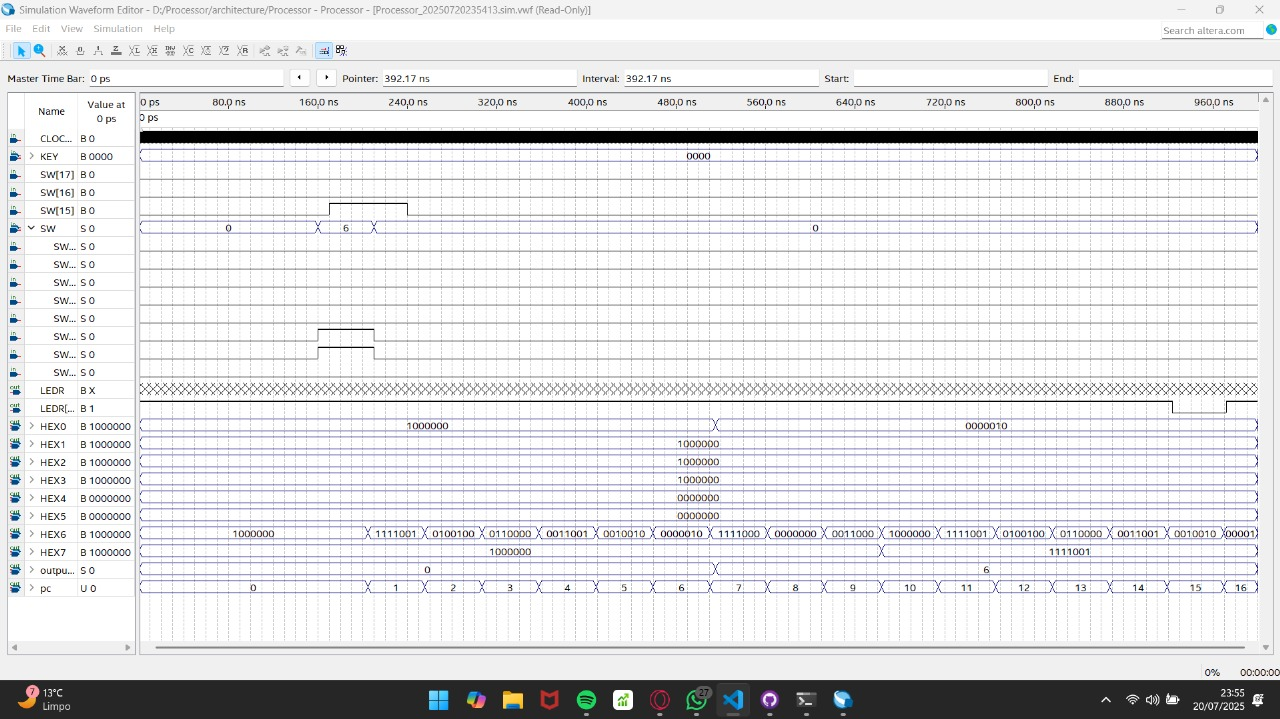
\includegraphics[width=\textwidth]{waveform.jpg}
    \legend{Fonte: O autor.}
\end{figure}

\newpage
\section{Exemplo 2: Contagem Regressiva Recursiva}
Este exemplo demonstra a capacidade do compilador de lidar com chamadas de função recursivas, um teste crucial para a correção da convenção de chamada e do gerenciamento da pilha.

\subsection{Código Fonte}
\begin{lstlisting}[language=C, caption={Código Fonte do Exemplo 2}]
void count (int number) {
  if(number == 0) return;
  output (number);
  count (number - 1);
}

int main (void) {
  int x;
  x = input();
  count(x);
}
\end{lstlisting}

\subsection{Código Intermediário}
O IR gerado mostra a estrutura da recursão: um caso base que leva a um \texttt{return} e um passo recursivo que inclui a chamada a \texttt{output} e a chamada a si mesmo com o argumento decrementado.
\begin{lstlisting}[language=text, caption={Código Intermediário do Exemplo 2}]
count:
  t0 := *number
  t1 := t0 == 0
  if_false t1 goto L0
  return _
L0:
  t2 := *number
  arg t2
  call output, 1
  t3 := *number
  t4 := t3 - 1
  arg t4
  call count, 1
  return _
main:
  t5 := call input, 0
  *x := t5
  t6 := *x
  arg t6
  call count, 1
  return _
\end{lstlisting}

\subsection{Código Assembly}
O código Assembly implementa o prólogo e o epílogo da função \texttt{count} para salvar e restaurar o registrador de link lógico (\texttt{lr}) e o ponteiro de frame (\texttt{fp}) na pilha a cada chamada.
\begin{lstlisting}[language=assembly, caption={Código Assembly do Exemplo 2}]
.text
.global main
    bi: main
count:
    subi: sp = sp, 1
    store: [sp] = lr
    subi: sp = sp, 1
    store: [sp] = fp
    mov: fp = sp
    mov: r4 = r1
    movi: r5 = 0
    subs: r0 = r4, r5
    bineq: count_L00
    bi: count_epilogue
count_L00:
    mov: r1 = r4
    out: r1
    subi: r6 = r4, 1
    mov: r1 = r6
    movi: lr = count_Lret0
    bl: count
count_Lret0:
    bi: count_epilogue
count_epilogue:
    mov: sp = fp
    load: fp = [sp]
    addi: sp = sp, 1
    load: lr = [sp]
    addi: sp = sp, 1
    b: lr
main:
    movi: sp = stack_space
    mov: fp = sp
    in: r4
    movi: r27 = 33
    store: [r27] = r4
    mov: r1 = r4
    movi: lr = main_Lret1
    bl: count
main_Lret1:
    bi: main_epilogue
main_epilogue:
    ret:

.data
stack_space: .space 64
var_x: .word 33
\end{lstlisting}

\newpage
\section{Exemplo 3: Ordenação por Seleção (Selection Sort)}
Este exemplo final demonstra a capacidade do compilador de lidar com um algoritmo mais complexo, envolvendo vetores, laços e chamadas de função aninhadas (`main` chama `sort`, que por sua vez chama `minloc`).

\subsection{Código Fonte}
\begin{lstlisting}[language=C, caption={Código Fonte do Exemplo 3}]
/* Ordenacao por selecao de uma matriz de dez elementos. */
int vet[10];

int minloc ( int a[], int low, int high )
{
    int i; int x; int k;
    k = low;
    x = a[low];
    i = low + 1;
    while (i < high) {
        if (a[i] < x) {
            x = a[i];
            k = i;
        }
        i = i + 1;
    }
    return k;
}

void sort( int a[], int low, int high)
{
    int i; int k;
    i = low;
    while (i < high-1) {
        int t;
        k = minloc(a,i,high);
        t = a[k];
        a[k] = a[i];
        a[i] = t;
        i = i + 1;
    }
}

void main(void)
{
    int i;
    i = 0;
    while (i < 10) {
        vet[i] = input();
        i = i + 1;
    }
    sort(vet,0,10);
    i = 0;
    while (i < 10) {
        output(vet[i]);
        i = i + 1;
    }
}
\end{lstlisting}

\subsection{Código Intermediário}
O IR para este exemplo é extenso, refletindo a complexidade do algoritmo. Ele demonstra a tradução de acesso a vetores em operações de cálculo de endereço por palavra: o índice é somado ao endereço base do vetor, sem multiplicação por 4, pois a RAM do processador é organizada em palavras de 32 bits. O mesmo trecho também exercita a passagem de múltiplos argumentos para as funções.
\begin{lstlisting}[language=text, caption={Código Intermediário do Exemplo 3 (trecho)}]
... (IR da funcao minloc omitido por brevidade)
sort:
  t27 := *low
  *i := t27
L4:
  t28 := *i
  t29 := *high
  t30 := t29 - 1
  t31 := t28 < t30
  if_false t31 goto L5
  t32 := *a
  arg t32
  t33 := *i
  arg t33
  t34 := *high
  arg t34
  t35 := call minloc, 3
  *k := t35
  t36 := *k
  t37 := &a
  t38 := t37 + t36
  t40 := *t38
  *t := t40
  ... (restante do IR omitido)
\end{lstlisting}

\subsection{Código Assembly}
O assembly gerado demonstra a implementação das principais funcionalidades do conjunto integrado entre compilador e processador.
\begin{lstlisting}[language=assembly, caption={Código Assembly do Exemplo 3 (esboço)}]
.text
.global main
    bi: main
minloc:
    subi: sp = sp, 1
    store: [sp] = lr
    subi: sp = sp, 1
    store: [sp] = fp
    mov: fp = sp
    ... (corpo da funcao minloc)
minloc_epilogue:
    mov: sp = fp
    load: fp = [sp]
    addi: sp = sp, 1
    load: lr = [sp]
    addi: sp = sp, 1
    b: lr
sort:
    subi: sp = sp, 1
    store: [sp] = lr
    ... (corpo da funcao sort, incluindo chamada para minloc)
    bl: minloc
sort_Lret0:
    ...
    bi: sort_epilogue
sort_epilogue:
    ...
    b: lr
main:
    movi: sp = stack_space
    mov: fp = sp
    ... (corpo da funcao main, incluindo chamada para sort)
    bl: sort
main_Lret0:
    ...
    bi: main_epilogue
main_epilogue:
    ret:

.data
stack_space: .space 64
var_vet: .word 34
... (outras variaveis globais)
\end{lstlisting}

\subsection{Análise Comparativa}
Este exemplo complexo destaca dois pontos fortes da fase de síntese:
\begin{enumerate}
    \item \textbf{Acesso a Vetores:} Uma expressão como \texttt{x = a[i];} é traduzida no IR para uma sequência de operações que calcula o endereço do elemento por palavra: obtém-se o endereço base do vetor, soma-se o índice e, finalmente, carrega-se o valor do endereço calculado. Essa escolha está alinhada à RAM de 32 bits por palavra usada no processador.
    \item \textbf{Chamadas Aninhadas:} A execução de \texttt{main} chama \texttt{sort}, que por sua vez chama \texttt{minloc}. O correto funcionamento depende do prólogo e epílogo de cada função, que salvam e restauram os registradores \texttt{lr} e \texttt{fp} na pilha. Isso garante que, quando \texttt{minloc} retorna, a execução continue corretamente dentro de \texttt{sort}, e quando \texttt{sort} retorna, a execução continue em \texttt{main}.
\end{enumerate}

%-------------------- Conclusão ---------------------
\chapter{Conclusão}
\label{cap:conclusao}

O desenvolvimento deste projeto consolidou a relação entre arquitetura de computadores e compiladores em um mesmo fluxo de trabalho. O processador ARM-like foi tratado como a base do sistema, com suas restrições concretas de instrução, memória, registradores e sinais de controle, enquanto o compilador C- foi adicionado como uma camada de software capaz de transformar programas de alto nível em código executável para essa arquitetura.

Uma das principais dificuldades encontradas na parte do compilador foi a construção da lógica para a geração da representação intermediária (IR). Por ser um conceito que precisei aprender e aplicar simultaneamente, o processo envolveu experimentação e retrabalho até que a estrutura do IR se tornasse robusta o suficiente para suportar as complexidades da linguagem e facilitar a subsequente geração de assembly.

Outro desafio significativo surgiu na fase de geração de código assembly e na sua compatibilização com o \texttt{Processor(v2026-1)}. Embora Python ofereça uma programação mais ágil em comparação com linguagens de mais baixo nível, a lógica de alocação de registradores, gerenciamento de pilha e tradução de instruções é inerentemente minuciosa. A coerência entre IR, assembly e formato binário exigiu análise cuidadosa para garantir que o assembly final estivesse correto e compatível com a arquitetura alvo.

Como destaque, a integração bem-sucedida entre o processador em Verilog, o front-end desenvolvido em C (com Flex e Bison), o gerador de IR, o back-end em Python, o montador e o simulador demonstrou a viabilidade de uma abordagem híbrida, aproveitando a força de cada tecnologia. A implementação de uma convenção de chamada funcional, com prólogo e epílogo para gerenciamento de pilha, passagem de argumentos, recursão e retorno em \texttt{r0}, foi um marco importante, permitindo a correta execução de funções aninhadas e recursivas. Este projeto não apenas resultou em uma ferramenta funcional, mas também proporcionou um aprendizado prático sobre a interação entre software, código de máquina e hardware.

Na versão atual documentada neste relatório, a integração com o \texttt{Processor(v2026-1)} ficou mais explícita: o texto diferencia branch imediato, branch por registrador e retorno por link dedicado, registra a RAM de 64 palavras e descreve como o binário final se relaciona com a ROM do projeto Quartus. Essa atualização reduz ambiguidades entre o compilador, o montador, o simulador em Python e o processador em Verilog.

% ----------------------------------------------------------
% ELEMENTOS PÓS-TEXTUAIS
% ----------------------------------------------------------
\postextual

% ----------------------------------------------------------
% Referências bibliográficas
% ----------------------------------------------------------
\bibliographystyle{abntex2-alf}
\bibliography{referencias}

\end{document}
